The interaction of light with any other object is described with a set of 
equations called the \emph{Maxwell equations}. This set of equations fully 
captures and describes the electromagnetic wave nature of light. These 
equations relate point wise the electric wave vector $\vb{E}$, the magnetic 
induction $\vb{B}$, the electric current density $\vb{J}$, the electric 
displacement $\vb{D}$, and the magnetic vector $\vb{H}$ with each other for 
objects where the physical properties are continuous in the neighbourhood of 
the point of interest~\cite{Born1980Ch1}
\begin{subequations}
  \begin{align}
    \curl{\vb{H}} - \frac{1}{\tilde{\speed}}\pdv{t}\vb{D} 
    &=\frac{4\pi}{c}\vb{J} \label{eq:TO-ampere} \\
    \curl{\vb{E}} + \frac{1}{\tilde{\speed}}\pdv{t}\vb{B} &=  0
    \label{eq:TO-faraday} \\
    \div{\vb{D}} &= 4\pi\rho_{\MR{E}}
    \label{eq:TO-gauss} \\
    \div{\vb{B}} &= 0
    \label{eq:TO-gauss-mag}
  \end{align}
\end{subequations}
with $\tilde{\speed}$ being the speed of light and $\rho_{\MR{E}}$ the total 
electric charge density. Although, 
\cref{eq:TO-ampere,eq:TO-faraday,eq:TO-gauss,eq:TO-gauss-mag} describe the 
behavior of light to great extent, it is often more convenient to think of 
light as a collection of single rays. The last missing equation to solve the 
stated problem fully is the material equation which describes the behavior of the 
material while being under the influence of the fields~\cite{Born1980Ch1}. In 
the limit of a vanishing small light wavelength $\lal$ compared to the object 
size $R$, the approximation of light as single rays is 
valid~\cite{Born1980Ch3}. This branch of optics describing the propagation of 
light is often called \emph{Ray Optics}.

Our laser has a wavelength of $\lal=\SI{785}{\nm}$ and the smallest object we 
use has a radius of $R=\SI{1.03}{\um}$. The ratio $\nicefrac{2R}{\lal}\approx 
2.6$ is close to unity and the application of ray optics in our case might be 
questionable. However, previous work with our optical trap
\cite{Lakaemper2015,Lamprecht2016,Lamprecht2017} has shown that the ray 
approximation is a reasonable approach for our setup.
% In addition, one has to differentiate between quantitative and qualitative 
% analysis. For most results in our thesis we use our optical trapping setup as 
% tool for relating results qualitatively.


\section{Experimental Setup}

\begin{figure}[tbp]
  \centering
  % \tikzsetnextfilename{setup}

  \definecolor{tempcolor}{RGB}{176, 206, 255}
\pgfmathdeclarefunction{gauss}{2}{%
  \pgfmathparse{1/(#2*sqrt(2*pi))*exp(-((x-#1)^2)/(2*#2^2))}%
}

\begin{tikzpicture}

  \shade[top color=white,bottom color=white,middle color=red] (3,-0.15) 
  rectangle ++(2.5,0.3);

  \shade[top color=white,bottom color=white,middle color=red] (5.5,-1.25) 
  rectangle (10,1.25);

  % laser head
  \filldraw[color=black,fill=black!50] (0,-0.5) rectangle ++(3,1);
  \node at (1.5,0) {Laser head};

  % lens
  \fill[tempcolor] (5.5,0) ellipse (0.15 and 1.5);
  \path (5,1.5) -- ++(1,0) node[above, midway, anchor=south] {Expanding lens};

  % microscope
  \filldraw[white] (9,-2) rectangle ++ (2,4);
  \filldraw[black] (9,-0.2) rectangle (9.2,-1.5);
  \filldraw[black] (9,0.2) rectangle (9.2,1.5);
  \filldraw[red] (9,-0.2) rectangle ++(1.5,0.4);

  \draw[black,thick] (10,-1) -- ++(0,0.8) -- ++(0.3,0) -- ++(0,0.4) -- 
  ++(-0.3,0) -- ++(0,0.8);

  \path (7.0,1.5) -- ++(4,0) node[above, midway, anchor=south, align=center] 
  {Microscope housing};

  \draw[black, very thick, ->] (11,0) -- ++(1.5, 0) -- ++(0, -4) -- ++(-1.5,0);

  \draw[black!70, thin] (7,-0.21) -- ++(2,0);
  \draw[black!70, thin] (7,+0.21) -- ++(2,0);

  %% bottom
  \fill[tempcolor] (10,-4) ellipse (0.15 and 0.75);
  \path (9.5,-3.25) -- ++(1,0) node[above, midway, anchor=south] {Focussing 
  lens};

  \coordinate (M) at (8.5,-4);
  \draw[black,thin,->] (M) -- node[above,pos=0.9] {\tiny$\ex$} ++(0,0.5);
  \draw[black,thin,->] (M) -- node[above,pos=0.9] {\tiny$\ey$} ++(0.4,0.4);
  \draw[black,thin,->] (M) -- node[above,pos=0.9] {\tiny$\ez$} ++(-0.5,0);
  \shade[ball color=black!10] (M) circle (.25);

  \path (8.25,-4.5) -- ++(0.5,0) node[below, midway] {particle};

  \fill[tempcolor] (7.0,-4) ellipse (0.15 and 0.75);
  \path (6.5,-3.25) -- ++(1,0) node[above, midway, anchor=south] {Condensor 
  lens};

  \filldraw[color=black, fill=black!50] (5.8,-4.5) rectangle ++(-1,1);
  \path (4.8,-4.5) -- ++(1,0) node[below, midway, anchor=north] {Filter};

  \fill[tempcolor] (2.5,-4) ellipse (0.15 and 0.75);
  \path (2,-3.25) -- ++(1,0) node[above, midway, anchor=south] {Lens 3};

  \filldraw[color=black, fill=black!10] (0,-4.4) rectangle ++(0.8,0.8);
  \draw[thick,black,dotted] (0,-4) -- ++(0.8,0);
  \draw[thick,black,dotted] (0.4,-4.4) -- ++(0,0.8);

  \path (0,-3.5) -- ++(0.8,0) node[above, midway, anchor=south] {QPDxy};
  \filldraw[color=red!50] (0.4,-4) circle (.2);

  \draw[red, thick] (11, -3.6) -- ++(-1,0) -- ++(-3,-0.8) -- (5.8,-4.4);
  \draw[red, thick] (11, -4.4) -- ++(-1,0) -- ++(-3,+0.8) -- (5.8,-3.6);
  \draw[red!50, thick, dashed]  (4.8,-4.4) -- (2.5,-4.4) -- (0.4,-3.8);
  \draw[red!50, thick, dashed]  (4.8,-3.6) -- (2.5,-3.6) -- (0.4,-4.2);

  % beam splitter
  \draw[gray,very thick] (3.2,-3.5) -- ++(1,-1);
  \path (3.2,-4.5) -- ++(1,0) node[below,midway] {Splitter};

  \fill[tempcolor] (3.7,-2.5) ellipse (0.75 and 0.15);
  \path (4.6,-2.5) -- ++(1,0) node[midway] {Lens 4};

  \filldraw[color=black, fill=black!10] (3.3,-2.0) rectangle ++(0.8,0.8);
  \draw[thick,black,dotted] (3.7,-2) -- ++(0,0.8);
  \draw[thick,black,dotted] (3.3,-1.6) -- ++(0.8,0);
  \path (2.9,-1.6) -- ++(-0.8,0) node[midway] {QPDz};

  \filldraw[color=red!50,opacity=0.3] (3.7,-1.6) circle (0.6);

  \draw[red!50, thick, dashed]  (3.3,-3.6) -- ++(0,1.1) -- (4.3,-2);
  \draw[red!50, thick, dashed]  (4.1,-4.4) -- ++(0,1.9) -- (3.1,-2);


\begin{axis}[
    domain=-0.15:0.15,
    samples=200,
    no markers,
    axis lines=none,
    ticks=none,
    xmin=-1,
    xmax=1,
    ymax=250,
    anchor = origin,
    rotate around={270:(current axis.origin)},
    hide axis,
    yshift=36mm
    ]

    \addplot[black] {gauss(0,0.01)};

\end{axis}

\begin{axis}[
    domain=-0.3:0.3,
    samples=100,
    no markers,
    axis lines=none,
    ticks=none,
    xmin=-1,
    xmax=1,
    ymax=20,
    anchor = origin,
    rotate around={270:(current axis.origin)},
    hide axis,
    yshift=65mm
    ]

    \addplot[black] {gauss(0,0.15)};

\end{axis}

\end{tikzpicture}

  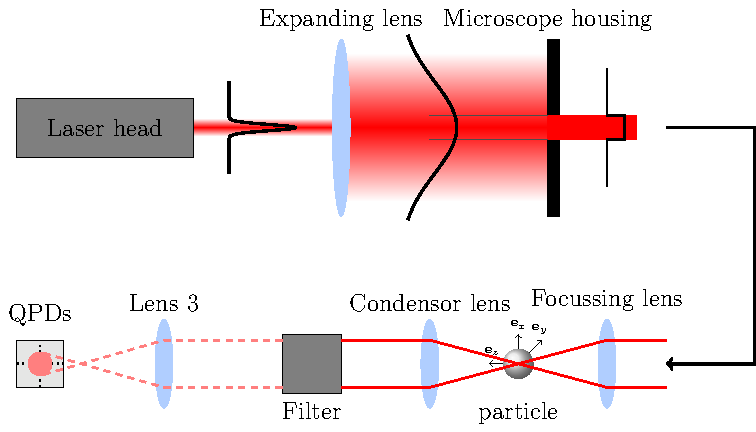
\includegraphics[]{/setup.pdf}
  \caption{Schematic of light path from laser head to quadrant photo detectors 
  (QPDs). In the top half red shading and the black lines outline the laser 
intensity profile qualitatively. In the bottom half just the most outer laser 
rays are depicted.}
  \label{fig:TO-setup}
\end{figure}

Before highlighting important parts from ray optics it is advantageous to 
understand our optical trapping setup which is based upon the work of Arthur 
Ashkin~\cite{Ashkin1978,Ashkin1987,Ashkin2002,Ashkin1986,Ashkin1992,Ashkin1997}. 
\cref{fig:TO-setup} depicts a basic schematic of the laser path from the laser 
source to the quadrant photo detectors (QPDs) in the back focal plane. A 
complete overview of our setup with a list and explanation of every used part 
is available in~\cite{Lamprecht2017}. In the following, we will highlight the 
path of the light from the laser source to the QPDs.

Our laser diode emits a tightly confined laser beam in the non-visible 
near-infrared regime with a wavelength of $\lal=\SI{785}{\nm}$ and a maximal 
power of $P=\SI{200}{\milli\watt}$. This laser profile is axisymmetric with 
respect to the light propagation direction and can be visualized with a 
rotating Gaussian bell curve (TEM$_{00}$). Next, the beam is expanded such 
that it is much larger than the opening of the microscope housing. The 
magnitude of the trapping forces are proportional to the laser intensity of the 
beam. The biggest contribution to the total trapping force stems from the outer 
parts of the beam because greater incident angles are present there. Therefore, 
the beam is broadened before guiding it to the focusing lens. The opening of 
the microscope is overfilled by the broadened beam such that the laser 
intensity is cut off and can be approximated with a flat-top profile. Hence, 
every light ray (also the ones contributing most to the total trapping force) 
carry the same power.

The next step is the focusing of the beam with a high numerical aperture (NA) 
oil immersion lens. At the focal point, the actual trapping of the particle 
occurs. If also the position of the trapped object relative to the focal point 
is of interest and not only the trapping of particles, the laser beam needs to 
be investigated further after the trapping. The relative particle movement 
within the trap changes the path of the beam ever so slightly that this 
deflection contains the necessary information for the movement analysis. In 
order to image the movement in all three spatial directions the beam is 
collimated again by the condensor lens after it passed by the particle and is 
filtered to reduce its total intensity to prevent damage of the QPDs. Before 
the beam is focussed, it is split into two parts because the axial movement 
detection for $\ez$ (QPDz) and the in plane movement detection for $\ex$ and 
$\ey$ (QPDxy) have inherently different working principles.

If the particle moves within the trap the spot on the QPDxy will also move. By 
measuring the voltage on each quadrant of the QPDxy and summing and subtracting 
certain quadrants it is possible to retrieve the information about the movement 
in each direction separately. For the axial direction the opening of the QPDz 
is overfilled. An axial movement of the particle causes a change of total 
intensity on this QPD. By measuring the QPDz total intensity we have the 
information about the relative particle movement within the trap along the 
axial $\ez$-direction~\cite{Felgner1995a}. For a conversion of the measured 
voltage to meter the OT needs to be calibrated.

In the following, we will always assume water as fluid medium and silicon 
dioxide (\SiO) as particle material. All calculations are also applicable to 
other fluid-particle material combinations with adapted material parameters.

\section{Optical Trap Calibration}

\begin{figure}[tbp]
  \centering
  % \tikzsetnextfilename{calibration}
%%%%%%%
% READ TABLE
%%%%%%%
{\small

\pgfdeclarelayer{background}
\pgfsetlayers{background,main}
\pgfplotstableread[col 
sep=comma]{\relPath/10_Figures/TikZ/12_ohneVerstaerker.dat}{\data}

\tikzstyle{lowpass}=[dashed, ultra thick, green!70!black]

\begin{tikzpicture}
\begin{loglogaxis}[
    width=140mm,
    height=70mm,
    title={FFT of Brownian Motion},
    xlabel={Frequency $f$ [Hz]},
    ylabel={Amplitude $A$ [Hz V$^{-2}$]},
    ymin=5e-14,
    ymax=1e-6,
    axis on top,
]

    \filldraw[black!10!white] (20,5e-14) rectangle (6000,1e-6);

    \addplot[thin] table[x=f, y=raw] {\data};
    \addlegendentry{raw};

    \addplot[red, thick] table[x=f, y=fit] {\data};
    \addlegendentry{fit};

    \draw[lowpass] ({axis cs:136,0}|-{rel axis cs:0,0}) -- (axis 
    cs:136,3.4289e-8) node [midway,right] {$f_c=136$};

    \draw[lowpass] ({axis cs:0,3.4289e-8}-|{rel axis cs:0,0}) -- (axis 
    cs:136,3.4289e-8) node[midway, above] {$A_{0}\approx \num{3.4e-8}$};

    \draw[lowpass] (axis cs:136,3.4289e-8) -- (axis cs:1e4,6.32e-12) 
    node[midway, sloped, above] {$\propto \nicefrac{1}{f^{2}}$};

\end{loglogaxis}
\end{tikzpicture}
}

  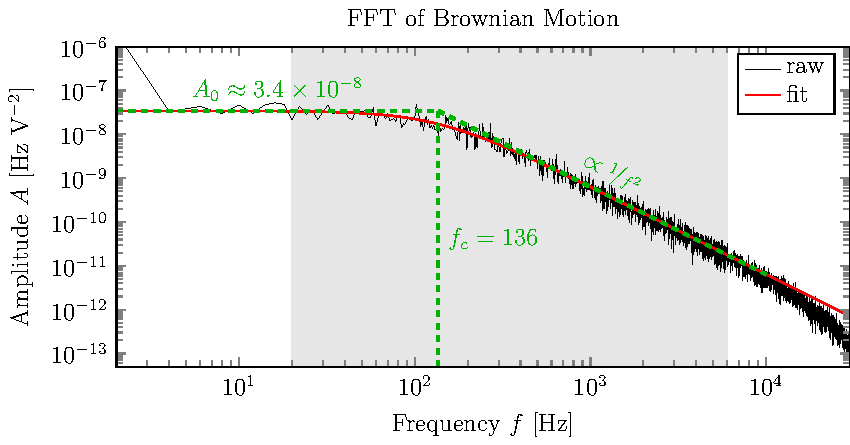
\includegraphics[]{External/calibration.pdf}
  \caption{Fast Fourier Transform (FFT) of over 10 cycles averaged Brownian 
    motion along the $\ex$ direction from a trapped \SiO~particle with of 
    $\SI{1.03}{\um}$. The gray shaded region \SIrange{20}{6000}{\hertz} depicts 
    the data points taken for the fit (\textcolor{red}{red}). The sampling 
  frequency of the DAQ system is \SI{1.25}{\mega\hertz} and the frequency 
resolution $\Delta f=\SI{2}{\hertz}$.}
  \label{fig:TO-calibration}
\end{figure}

There exist different methods to calibrate an OT. A discussion of different 
calibration options is available from \cname{Svoboda1994} and \cname{Jun2014}. 
Our calibration is based on the passive power spectrum of a trapped particle 
that is still moving due to Brownian motion. The motion of the trapped particle 
is described by
\begin{equation}
  \gamma\dot{q_{i}} + \kappa_{i}q_{i} = \FLangevin(t)
  \label{eq:TO-cal-eom}
\end{equation}
where $q_{i}$ is the position of the trapped particle along any of the 
orthogonal directions $\ex, \ey$ and $\ez$, $\gamma$ is Stokes' drag 
coefficient, $\kappa_{i}$ the stiffness of the OT, and $\FLangevin(t)$ the time 
dependent Langevin force. The correction by including the inertia term 
$m\ddot{q_{i}}$ for the calculation is negligible small because the particle 
masses are negligible small.

By solving \cref{eq:TO-cal-eom} in the frequency domain
\begin{equation}
  \hat{q}_{i}(f) = \frac{\hat{F}_{\MR{Langevin}}}{\gamma\left( 2\pi \cutoff - 
  \iu 2\pi f \right)}
  \label{eq:TO-cal-Fdomain}
\end{equation}
where $\hat{\Box}$ denotes a quantity in the frequency domain and $\cutoff$ the 
cut off frequency. Taking the Lorentzian power spectrum of 
\cref{eq:TO-cal-Fdomain} and using the relation
\begin{equation}
  \abs{\hat{F}_{\MR{Langevin}}}^{2} = 2\,\gamma\,k_{\MR{Bo}}T
\end{equation}
where $T$ is the temperature and $k_{\MR{Bo}}$ the Boltzmann constant one finds 
\begin{equation}
  \mathcal{F}_{i}=\frac{k_{\MR{Bo}}T}{2\pi^{2}\gamma\left( \cutoff^{2}+ f^{2} 
  \right)}
\end{equation}
where $\mathcal{F}_{i}$ is the Lorentzian power spectrum~\cite{Lamprecht2017}. 
The power spectrum of the trapped particle resembles the curve of a lowpass 
filter and can, hence, be fitted to
\begin{equation}
  \mathcal{F}_{\MR{Lowpass}}(f) = \frac{A_{0}}{f^{2} + \cutoff^{2}}
\end{equation}
where $A_{0}$ is the amplitude at $f=0$. \cref{fig:TO-calibration} depicts the 
Fast Fourier Transform (FFT) of the Brownian motion along $\ex$ of a trapped 
\SiO~particle with \SI{1.03}{\um} radius and water as surrounding medium, as 
well as, the fitted lowpass curve and its fitting parameter. The FFT and the 
fit of the Brownian motion along $\ey$ is very similar to the depicted one 
because the in-plane optical potential is axissymmetric to $\ez$. Since it is 
known, that the OT is weaker along the axial $\ez$ direction, a FFT of the 
Brownian motion along $\ez$ looks qualitatively the same to the one in 
\cref{fig:TO-calibration} but shifted a little to lower frequencies; hence, the 
respective $\cutoff$ frequency is also less.

With the fitting parameters $A_{0}$ and $\cutoff$ it is possible to calculate 
the stiffness of the OT
\begin{equation}
  \kappa_{i} = 2\pi\,\gamma\,\cutoff,
\end{equation}
as well as the conversion factor
\begin{equation}
  \Upsilon_{i} = \frac{1}{\pi\cutoff}\,
  \sqrt{\frac{k_{\MR{Bo}}T}{\gamma A_{0}}}
  \label{eq:TO-cal-Upsilon}
\end{equation}
which has the unit [\si{\meter\per\volt}] and converts the measured voltage at 
the QPDs to a particle displacement relative to the trap center. For 
\cref{eq:TO-cal-Upsilon} the Equiparation Thoerem~\cite{Wang1945} is utilized 
which relates the product of the time-averaged variance of the trapped particle 
position with the OT stiffness to its energy content.
\begin{equation}
  \kappa_{i}\,\timeaverage{q_{i}^{2}} = k_{\MR{Bo}}T.
\end{equation}



to the energy content.
\section{Ray Optics\label{sec:TO-rayoptics}}

As mentioned before, in the regime of ray optics the propagation of light is 
visualized by single rays. The interaction of a single ray at an interface is 
then studied geometrically. The defining property for ray optics is the so 
called refractive index $\refraction$. Light travels at the speed of light 
$\tilde{\speed}=\SI{299792458}{\m\per\s}$ in vacuum. Outside of vacuum the 
speed of light has a smaller magnitude. The refractive index relates the speed 
of light of vacuum $\tilde{\speed}$ to the speed in any other material 
$\tilde{\speed}_{\Box}$
\begin{equation}
  \tilde{\speed}_{\Box} = \frac{\tilde{\speed}}{n_{\Box}}.
  \label{eq:TO-lightspeed}
\end{equation}
Since there is nothing faster than the speed of light in vacuum, the refractive 
index $\refraction$ cannot be smaller than 1. This index is not constant for 
one material but a function of the wavelength $\lal$. Additionally, the 
refractive index is in general a complex quantity
\begin{equation}
  \abs{\refraction}\geq 1 \quad \wedge \quad \refraction \coloneqq 
  \refraction(\lal) = \nreal(\lal) - \iu \nimag(\lal)
  \label{eq:TO-refractive-index}
\end{equation}
where $\nimag$ is called the extinction coefficient~\cite{Jackson2013}. The 
absorption coefficient for the light intensity~\cite{Hecht2017}
\begin{equation}
  \alpha = \frac{4\pi f \nimag}{\tilde{\speed}} = 
  \frac{4\pi}{\lal}\nimag\quad\text{with}\quad\lal=\frac{\tilde{\speed}}{f}
  \label{eq:TO-alpha}
\end{equation}
converts the dimensionless quantity $\nimag$ into a physical parameter with 
unit \si{\per\meter} and is a measure for the absorbed energy per distance; a 
higher value implies higher absorption per traveled distance. After a distance 
of $\alpha\left(\lal\right)^{-1}$ the ray intensity with wavelength $\lal$ 
decreased by 63.2\%. \Cref{fig:TO-n_water} depicts $n$ and $\alpha$ of water 
for different wavelengths $\lal$. Whereas the real part of the refractive index 
is about constant for $\lal > \SI{400}{\nm}$, the absorption coefficient 
changes its value over 4 orders of magnitude in the same interval.

\begin{figure}[tbp]
  \centering
  % \tikzsetnextfilename{n_water}
%%%%%%%
% READ TABLE
%%%%%%%

\begin{tikzpicture}
\begin{axis}[
  height=80mm,
  width=120mm,
  no markers,
  xlabel={$\lal$ [\si{\nm}]},
  ylabel={$\nreal$ [-]},
 ]

    \addplot[black] table[x=wl,y=n] 
    {\relPath/10_Figures/TikZ/Segelstein1981a.dat};

    \label{plot_n}
    \draw[dashed,<->,latex-latex] ({axis cs:785,0}|-{rel axis cs:0,0.0}) -- 
    (785,1.326244) -- node[above,pos=0.65,fill=white,opacity=0.8,text 
    opacity=1] {\footnotesize 1.326} ({0,1.326244}-|{rel axis cs:0,0});
\end{axis}
\begin{axis}[
  height=80mm,
  width=120mm,
  axis y line*=right,
  axis x line=none,
  ylabel={$\alpha$ [\si{\per\meter}]},
  no markers,
  ymode = log,
]
    \addlegendimage{/pgfplots/refstyle=plot_n}\addlegendentry{$\nreal$}
    \addplot[black,dash dot] table[x=wl,y=a] 
    {\relPath/10_Figures/TikZ/Segelstein1981a.dat};
    \addlegendentry{$\alpha$}

    \draw[dashed,<->,latex-latex] ({axis cs:785,0}|-{rel axis cs:0,0.0}) -- 
    (785,2.144) -- node[above,pos=0.73] {\footnotesize 2.144} 
    ({0,2.144}-|{rel axis cs:1,0});
    % 2.14353e+00

    \draw[dotted,<->,latex-latex] ({axis cs:1060,0}|-{rel axis cs:0,0.0}) -- 
    (1060,15.40) -- node[above,pos=0.53,fill=white,opacity=0.8,text 
    opacity=1] {\footnotesize 15.40} ({0,15.40}-|{rel axis cs:1,0});
    % 1.53991e+01
\end{axis}
\end{tikzpicture}

  \includegraphics[]{/n_water.eps}
  \caption{Index of refraction $\nreal$ and absorption coefficient $\alpha$ for 
  water over the wavelength $\lal$. Data taken from 
\cite{Hale1973,Segelstein1981}.}
  \label{fig:TO-n_water}
\end{figure}


Any ray of any wavelength is attenuated when propagating through a medium. The 
\emph{Beer-Lambert Law}
\begin{equation}
  \intensity(s) = \intensity_{0}\exp(-\alpha s)
  \label{eq:TO-beer-lambert}
\end{equation}
captures the change of intensity while moving along the path $s$ where 
$\intensity_{0}$ is the intensity at the start of the path. E.g. in a depth of 
approximately \SI{1}{\kilo\meter} it is completely dark in the ocean because 
all the intensity of the sunlight is attenuated there.

\begin{figure}[tbp]
  \centering
  % \tikzsetnextfilename{Snell}

\tikzstyle arrowstyle=[scale=1]

\tikzstyle directed=[postaction={decorate,decoration={markings,
    mark=at position .65 with {\arrow[arrowstyle]{stealth}}}}]

\tikzstyle reverse directed=[postaction={decorate,decoration={markings,
    mark=at position .65 with {\arrowreversed[arrowstyle]{stealth};}}}]

\tikzset{SnellNode/.style={text width=10mm, align=center}}

\begin{tikzpicture}
  \def\W{5}
  \def\H{4}
  \def\x{0.95}
  \def\anglealpha{0}
  \pgfmathsetmacro{\y}{{(1-\x)*\H}}
  \pgfmathsetmacro{\radius}{(\W^2+\y^2)/2/\y}
  \pgfmathsetmacro{\anglealpha}{{asin(\W/\radius)}}
  \pgfmathsetmacro{\s}{{90+\anglealpha}}
  \pgfmathsetmacro{\e}{{90-\anglealpha}}

  \pgfmathsetmacro{\anglebeta}{{0.8*\anglealpha}}
  \pgfmathsetmacro{\p}{{(\radius-\H)*sin(\anglebeta)}}
  \pgfmathsetmacro{\px}{{\radius*sin(\anglebeta)}}
  \pgfmathsetmacro{\py}{{-\radius*(1-cos(\anglebeta))}}


  % define coordinates
  \coordinate (O) at (0,0) ;
  \coordinate (A) at (0,\H) ;
  \coordinate (B) at (0,-\H) ;

  % media
  \fill[blue!20,opacity=.3] (-\W,0) rectangle (\W,\H);
  \fill[black!10!,opacity=.3] (-\W,0) rectangle (\W,-\H);
  \node[right, SnellNode] at (2,1.5) {{Fluid\\ $\nf$}};
  \node[left, SnellNode] at (-2,-2) {{Particle\\ $\ns$}};

  % axis
  \draw[dash pattern=on5pt off3pt] (A) -- (B) ;
  % normal
  \draw[|->, thick] (0,0) -- node[right, pos=1] {$\normalvector$} (0, 2.5);


  % ray representation
  \def\gamma{130}
  \draw[red, variable=\x, domain=2.5:\W, samples=100] (0,\H) plot 
  ({\x*cos(\gamma)-cos(\x*pi r*3)/4*sin(\gamma)},{sin(\gamma)*\x+cos(\x*pi 
  r*3)/4*cos(\gamma)});

  % rays
  \draw[red,ultra thick,reverse directed] (O) -- node[left, xshift=-1mm, 
  pos=0.2] {$P_{\mathrm{i}}$} (130:5.2);

  \draw[red,ultra thick,directed] (O) -- node[right, xshift=1mm, pos=0.2] 
  {$P_{\mathrm{r}}$} (50:5.2);

  \draw[blue,directed,ultra thick] (O) -- node[right, xshift=1mm, pos=0.2] 
  {$P_{\mathrm{t}}$} (-70:4.24);

  % particle circumference
  \draw (-\W,-\y) arc (\s:\e:\radius);
  \draw[black,->|,>=stealth'] (\p,-\H) -- node[right, pos=0.7] {$\R$} (\px, 
  \py);

  % angles
  \draw[->,>=stealth'] (0,1) arc (90:130:1);
  \draw[->,>=stealth'] (0,1) arc (90:50:1);
  \draw[->,>=stealth'] (0,-1.4) arc (270:290:1.4);

  \node[] at (280:1.8)  {$\transmitted$};
  \node[] at (110:1.4)  {$\incident$};
  \node[] at (70:1.4)  {$\refracted$};

\end{tikzpicture}

  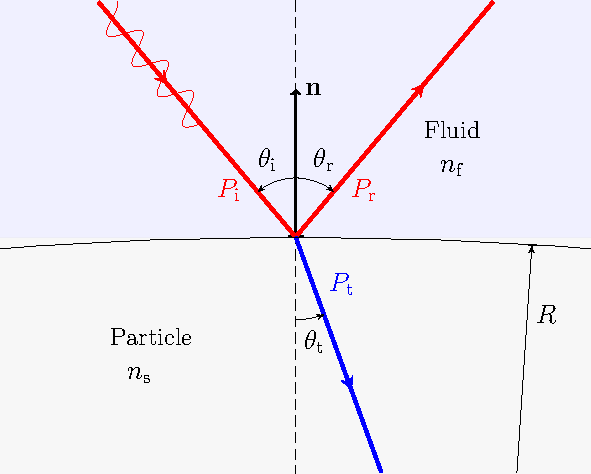
\includegraphics[]{/Snell.pdf}
  \caption{Visualization of Snell's Law for rays at an interface of two media 
  with different refractive indices $\refraction_{\Box}$.}
  \label{fig:TO-Snell}
\end{figure}

With the real part of the complex refractive index $\refraction(\lal)$, it is 
possible to define the most important relation in the ray optics regime: 
\emph{Snell's Law} (see also \cref{fig:TO-Snell}) is
\begin{equation}
  \nf\,\sin\incident = \ns\,\sin\transmitted.
  \label{eq:TO-Snell}
\end{equation}
This law connects the angle of incident $\incident$ with the transmitted angle 
$\transmitted$ at an interface of two different media with refractive indices 
$\nf$ and $\ns$, respectively. This law is based on the fact that a ray of 
light travels on the fastest and not the shortest path between two 
points~\cite{Born1980Ch3}. The angle of the reflected ray is equal to the 
incident angle ($\reflected=\incident$).

Another angle of special interest is the angle of total internal reflection 
% $\theta_{\MR{TIR}}$
\begin{equation}
  \theta_{\MR{TIR}}=\sin^{-1} \frac{\ns}{\nf}
  % \incident \quad \text{}\forall\quad \frac{\nf}{\ns}\,\sin\incident > 1.
  \label{eq:TO-TIR}
\end{equation}
For incident angles of this magnitude or greater 
($\incident\geq\theta_{\MR{TIR}}$), no ray is transmitted into the other 
medium; only reflection is occurring. It can only occur if the index of 
refraction of the incident medium is greater than the transmitted medium 
($\nf>\ns$ in \cref{fig:TO-Snell}) otherwise the ratio $\sfrac{\nf}{\ns}$ of 
\cref{eq:TO-TIR} is always smaller than unity and there is physically no total 
internal reflection possible.

% The other angle of special interest is the so called \emph{Brewster Angle} 
% $\theta_{\MR{B}}$
% \begin{equation}
  % \theta_{\MR{B}} = \tan^{-1}\left( \frac{\ns}{\nf} \right).
  % \label{eq:TO-brewster}
% \end{equation}
% At this angle there does not occur an reflection and hence all the intensity is 
% transmitted.

\cref{eq:TO-Snell} calculates in which direction a ray will travel after an 
interface of two media. The intensity amplitude of the reflected and 
transmitted rays can be computed with the so called \emph{Fresnel 
Equations}~\cite{Jackson2013,Born1980Ch1}. Although we think of light as rays, 
the theory behind those equations is based on the electromagnetic wave 
character of light. For time harmonic electromagnetic waves the amplitude of 
the incident electric wave vector $\abs{\vb{E}_{\MR{i}}}$ to the transmitted 
electric wave vector $\abs{\vb{E}_{\MR{t}}}$ and to the reflected electric wave 
vector $\abs{\vb{E}_{\MR{r}}}$ is related by $\fresnelr_{i}$ and 
$\fresnelt_{i}$ at the interface of the two media
\begin{subequations}
\begin{align}
  \abs{\vb{E}_{\MR{r}}} & =\fresnelr_{i}\,\abs{\vb{E}_{\MR{i}}} \\[3mm]
  \abs{\vb{E}_{\MR{t}}} & =\fresnelt_{i}\,\abs{\vb{E}_{\MR{i}}}
\end{align}
\end{subequations}
where the subscript $i$ can either be $i=\MR{p}$ for p-polarized light or 
$i=\MR{s}$ for s-polarized light~\cite{Jackson2013,Born1980Ch1}. ``p'' and 
``s'' stand for the German words ``parallel'' (parallel) and ``senkrecht'' 
(perpendicular), respectively. They refer to the orientation of the incident 
electric field $\vb{E}_{\MR{i}}$ to the plane of incidence. For the special 
cases of ``p'' and ``s'' polarized light the Fresnel coefficient with the 
assumption that both media are non-magnetic ($\mu_{\MR{f}} = \mu_{\MR{s}} = 
\mu_{0} = 1$)~\cite{Born1980Ch1} are
\begin{subequations}
\begin{align}
  \fresnelr_{\MR{s}} & =
  \frac{2\,\nf\,\cos\incident}{\nf\,\cos\incident + \ns\,\cos\reflected} 
  \label{eq:TO-fresnel-rs}\\[3mm]
  \fresnelt_{\MR{s}} & = \frac{\nf\,\cos\incident - 
  \ns\,\cos\reflected}{\nf\,\cos\incident + \ns\,\cos\reflected} 
  \label{eq:TO-fresnel-ts}\\[3mm]
  \fresnelr_{\MR{p}} & =
  \frac{2\,\nf\,\cos\incident}{\ns\,\cos\incident + \nf\,\cos\reflected} 
  \label{eq:TO-fresnel-rp}\\[3mm]
  \fresnelt_{\MR{p}} & = \frac{\ns\,\cos\incident - 
  \nf\,\cos\reflected}{\ns\,\cos\incident + \nf\,\cos\reflected}.
\label{eq:TO-fresnel-tp}
\end{align}
\end{subequations}
The Fresnel coefficients relate the amplitudes of the transmitted and reflected 
electrical field to the incident electrical field. In general, the sum of 
$\fresnelr_{i}$ and $\fresnelt_{i}$ does not add up to one.

For \cref{sec:TO-temperature}, it is necessary to know how much of the incident 
power $P_{\MR{i}}$ is transmitted and how much is reflected. The power 
$P=\intensity A$ is a product of the intensity $\intensity$ and the area $A$ 
the power is acting on. The intensity is defined as the time-average of the 
Poyting vector $\vb{S}$
\begin{equation}
  \intensity = \timeaverage{\abs{\vb{S}}} = 
  \timeaverage{\abs{\vb{E}_{0}\times\vb{H}_{0}}} = 
  \frac{1}{2}\,\frac{\refraction}{Z_{0}}\,\abs{\vb{E}_{0}}^{2} = 
  \frac{1}{2}\,\refraction\,c\epsilon_{0}\,\abs{\vb{E}_{0}}^{2}
\end{equation}
where $Z_{0}$ is the electrical impedance of free space and $\epsilon_{0}$ is 
the vacuum permittivity. With 
\cref{eq:TO-fresnel-rs,eq:TO-fresnel-ts,eq:TO-fresnel-rp,eq:TO-fresnel-tp} the 
amplitudes of the electrical fields at the interface are defined. With the 
relation for the distance $w$ of two parallel rays at the interface (see also 
\cref{fig:TO-Snell})
\begin{equation}
  w = \frac{w_{\MR{i}}}{\cos\incident} = \frac{w_{\MR{r}}}{\cos\reflected} = 
  \frac{w_{\MR{t}}}{\cos\transmitted}
  \label{eq:TO-area}
\end{equation}
and the scaling of the power
\begin{equation}
  P = \intensity A \propto \refraction\,\abs{\vb{E}_{0}}^{2}A \propto
  \refraction\,\abs{\vb{E}_{0}}^{2}w_{\Box}
\end{equation}
one can calculate the reflectance $\fresnelR_{i}$ as the ratio of the reflected 
power $P_{\MR{r}}$ to the incident power $P_{\MR{i}}$ as
\begin{equation}
  \fresnelR_{i} = \frac{P_{\MR{r}}}{P_{\MR{i}}} = 
  \frac{\intensity_{\MR{r}}\,\nf\,w_{\MR{r}}}{\intensity_{\MR{i}}\,\nf\,w_{\MR{i}}} 
  =\frac{\abs{\fresnelr_{i}\,\vb{E}_{0}}^{2}}{\abs{\vb{E}_{0}}^{2}} = 
  \fresnelr_{i}^{2}
  \label{eq:TO-fresnelR}
\end{equation}
where again the italic $i$ in the subscript ($\Box_{i}$) indicates the 
polarization. Similarly one finds the transmittance $\fresnelT_{i}$ as
\begin{equation}
  \fresnelT_{i} = \frac{P_{\MR{t}}}{P_{\MR{i}}} = 
  \frac{\intensity_{\MR{t}}\,\ns\,w_{\MR{t}}}{\intensity_{\MR{i}}\,\nf\,w_{\MR{i}}} 
  =\frac{\abs{\fresnelt_{i}\,\vb{E}_{0}}^{2}}{\abs{\vb{E}_{0}}^{2}}\,\frac{\ns\,w_{\MR{t}}}{\nf\,w_{\MR{i}}} 
  = \fresnelt_{i}^{2}\,\frac{\ns\,\cos\transmitted}{\nf\,\cos\incident}.
  \label{eq:TO-fresnelT}
\end{equation}
For unpolarized rays one can take the arithmetic average of $\Box_{\MR{s}}$ and 
$\Box_{\MR{p}}$ polarization values. Other than the Fresnel coefficients the 
sum of the reflectance $\fresnelR$ and the transmittance $\fresnelT$ for one 
angle of incidence need to be unity
\begin{equation}
  \fresnelR + \fresnelT = 
  \frac{\fresnelR_{\MR{s}}+\fresnelR_{\MR{p}}}{2} +
  \frac{\fresnelT_{\MR{s}}+\fresnelT_{\MR{p}}}{2} = 1 
  \label{eq:TO-fresnel}
\end{equation}
because the incident power $P_{\MR{i}}$ is either reflected or transmitted
\begin{equation}
  P_{\MR{i}} = P_{\MR{r}} + P_{\MR{t}} = P_{\MR{i}}\left( \fresnelR + \fresnelT 
  \right).
\end{equation}

\section{Laser Induced Temperature Change\label{sec:TO-temperature}}

A laser is a coherent beam of electromagnetic waves of a single wavelength 
$\lal$. Intensities with the orders of \si{\mega\watt\per\square\meter} and 
more are common. For comparison, the average intensity of the sun on to the 
earth in Central Europe is about \SI{1.36}{\kilo\watt\per\square\meter}, and 
the laser of our setup has with its peak power of \SI{200}{\milli\watt} and a 
specified beam diameter of \SI{1}{\mm} a maximal intensity of about 
\SI{0.25}{\mega\watt\per\square\meter}. As described with the Beer-Lambert-Law
(\cref{eq:TO-beer-lambert}) some of the laser intensity is attenuated while 
traveling through a medium. The attenuation of intensity will lead to an 
increase of temperature in the absorbing medium and, hence, to a change of the 
viscosity in the fluid. This viscosity change might lead to wrong force 
measurement results because the calibration parameters $\kappa_{i}$ and 
$\Upsilon_{i}$ and, therefore, the absolute measured force dependent on the 
fluid viscosity.

The intensity of a focused laser is highest in the region of the focal point 
because all of its power is confined to a small area with a width of about one 
wavelength. Direct temperature measurements in the vicinity of the focussed 
laser and the particle are up to now not possible due to the microscopic region 
of interest up. Precise knowledge of the temperature change is not only of 
interest for the calibration process of the OT but also for objects that need 
to stay below a certain temperature, e.g. living cells.

We tried unsuccessfully to measure the laser induced temperature change with 
temperature sensors that were sputtered onto the bottom of the channel by 
\cname{Werr2019}. However, the material of those sensors were layers in the 
\si{\nm} range of titanium and platinum. Both materials have optical absorption 
coefficients $\alpha$ at our laser wavelength which are about 7 orders of 
magnitude greater than the absorption coefficient of water. In order to utilize 
these kind of sensors the distance between the OT focal point and the sensors 
must be large enough such that no rays are hitting the sensor surface. If rays 
are hitting the sensor surface the measured temperature increase is due to the 
heating of the sensor itself and not the effect of a changed temperature of the 
surrounding fluid. At distances where it is expected that no laser ray will hit 
any sensor surface the expected temperature increase is so little that it 
cannot be distinguished from noise in the data of the measurement and is, 
hence, not conclusive.

Therefore, we will first discuss in the following sections the current research 
regarding temperature increase in OTs, discuss the path of a ray through the 
particle, and then motivate a temperature calculation based on simple ray 
optics that can approximate the laser induced heating at the focal point in the 
trapped particle for our experimental setup.

\subsection{State of the Art}\label{sec:TO-state}

\cyear{Liu1995} measured the temperature dependent change in the fluorescence 
of biological cells while being trapped with a wavelength of 
$\lal=\SI{1064}{\nm}$. They found a linear relation between temperature 
increase and applied laser power of about \SI{15}{\degreeCelsius\per\watt}. In 
addition, they solved the heat problem also analytically. For that, they 
neglected the trapped object and modeled it as water because their cells of 
interest consisted mainly of water. The experiments as well as the analytical 
solution show an almost instantaneous change in temperature after the laser was 
switched on.

\cyear{Celliers2000} measured the local change in the index of refraction for 
water while being subjected to a laser with a wavelength of \SI{985}{\nm}. 
During the measurements no objects were trapped in the laser focus. They 
measured a temperature increase of \SI{4}{\degreeCelsius} with a laser power of 
\SI{55}{\milli\watt} in the focus of the laser leading to a heating coefficient 
of \SI{72}{\degreeCelsius\per\watt}. An analytical model that utilized an 
improved source term compared to \cite{Liu1995} validated their results.

\cyear{Peterman2003} measured with a OT of $\lal=\SI{1064}{\nm}$ wavelength the 
effects of the temperature increase in the vicinity of the laser focus. A 
change of temperature in the fluid will lead to a change of the fluid 
viscosity. The viscosity change alters the calibration parameters of the OT. By 
fitting the calibration parameters for different laser powers to the 
theoretical relation they found a temperature increase of roughly 
\SI{8}{\degreeCelsius\per\watt} for water as fluid medium and silica beads as 
trapped objects. More interestingly, their analytical model revealed that most 
of the heat absorption is in the fluid rather than the trapped object. In 
addition, usual glass coverslips act as fast heat conductor compared to water 
such that measurements close to the top or bottom surface of the fluid cavity 
lead to a less temperature increase than in the bulk of the fluid.

\cyear{Moreau2015} injected Rhodamine B (RhB) in cells to measure the 
temperature change of an OT with $\lal=\SI{800}{\nm}$ wavelength. RhB is a 
temperature sensitive dye which changes its fluorescence linearly with the 
temperature. Since they injected the RhB into the cell the measured 
temperature difference was close to the focal point. As before, the increase of 
the temperature occurred almost instantaneously and was about 
\SI{9}{\degreeCelsius\per\watt}.

Lastly, in \citeyear{Catala2017}, \cname{Catala2017} studied the effects of 
different experimental parameters (NA, material of trapped object, distance to 
coverslips, object radius) to the magnitude of the temperature increase with an 
OT of $\lal=\SI{1064}{\nm}$ wavelength. A numerical model validated their 
experimental findings. Their source term which is an extension to 
\cname{Peterman2003} took account of the NA, the finite focal spot size, and 
the wavelength of the laser itself. In agreement to the others they found the 
heat increase to be about \SI{20}{\degreeCelsius\per\watt}.

All of the aforementioned studies (see also \cref{tab:TO-heating}) validated in 
their experiments the linear relation of the applied laser power to the 
increase in temperature. Also, they showed that the temperature change occurs 
almost instantaneously and that a steady state without any further temperature 
increase is established in the range of a few \si{\ms}. In addition, they agree 
that the main absorption occurs in the fluid medium (water or glycerol) rather 
than the trapped object itself because the absorption coefficient of the fluid 
$\alpha_{\MR{f}}$ is greater than of the particle $\alpha_{\MR{s}}$ for PS or 
silica. Besides \cname{Moreau2015} and \cname{Celliers2000} all studies operate 
at a wavelength of \SI{1064}{\nm}. Our OT operates at \SI{785}{\nm} and the 
absorption coefficient $\alpha_{\MR{f}}$ for this wavelength and for water is 
about one order of magnitude smaller than it is at \SI{1064}{\nm},
$\alpha_{\MR{f}}(\SI{785}{\nm}) \approx \SI{2.14}{\per\meter} $ and 
$\alpha_{\MR{f}}(\SI{1064}{\nm}) \approx \SI{15.4}{\per\meter} $ respectively 
(see \cref{fig:TO-n_water}).
% The magnitude of the absorption coefficient $\alpha_{\MR{f}}$ is the measure 
% for how much power gets absorbed by the fluid.
% The parameter $\alpha_{\MR{f}}$ contributes linear to the source term in the 
% heat equation.

Besides the results of \cname{Peterman2003} the measured temperature increase 
is larger for the wavelength of \SI{1064}{\nm}. The magnitudes of the 
respective absorption coefficients $\alpha_{\Box}$ 
($\nicefrac{15.4}{2.14}\approx 7.2$) suggest a seven times greater heating for 
the \SI{1064}{\nm} wavelength. However, only the results of 
\cname{Celliers2000} compared to \cname{Moreau2015} match this interpolation. 
But \cname{Celliers2000} used an inherently different method for approximating 
the temperature increase where no object was trapped during the measurement. 
Despite having contradicting results, we take a heating value of 
\SI{10}{\degreeCelsius\per\watt} for water and our wavelength of \SI{785}{\nm} 
as given for the following section if the focus of the OT is at least 
\SI{10}{\um} away from any surrounding surface. With a peak power of 
$\SI{0.2}{\watt}$ the water temperature will not increase by more than 
\SI{2}{\degreeCelsius} for our OT setup.

\begin{table}
  \centering
  \begin{tabular}{l *{6}{c}}
    \toprule
    \toprule
    Author & $\lambda$ & Heating & Mat. & Exp. & Ana. & Num. \\
    & [\si{\nm}] & [\si{\degreeCelsius\per\watt}] \\
    \midrule
    \cname{Liu1995} & 1064 & 15 & Cells & $\checkmark$ & $\checkmark$ & \\
    \cname{Peterman2003} & 1064 & 8 & Si & $\checkmark$ & $\checkmark$ & \\
    \cname{Catala2017} & 1064 & 20 & Si & $\checkmark$ & $\checkmark$ & 
    $\checkmark$ \\
    \cname{Celliers2000} & 985 & 72 & - & $\checkmark$ & $\checkmark$ & \\
    \cname{Moreau2015} & 800 & 9 & Cells & $\checkmark$ & & \\
    \bottomrule
    \bottomrule
  \end{tabular}
  \caption{Overview of studies to laser induced heating in OTs. Mat.=Material 
  type of the trapped object, Ex.=Experimental part, Ana.=Analytical model, 
Num.=Numerical model}\label{tab:TO-heating}
\end{table}

\subsection[Ray Path \& absorbed Energy]{Ray Path through Particle and absorbed 
Energy}

Before approximating the heat distribution inside the trapped particle with ray 
optics, it is necessary to investigate the path of the ray through the 
particle. In \cref{fig:TO-ray_particle} a ray with power $\power{i}{1}$ is 
incident on the particle surface in point $A$. The direction of the ray is 
towards the focal point $f$ which is slightly above the middle point $M$ of the 
particle because the stable trapping position is the equilibrium of the 
trapping forces towards the point $f$, the repulsive radiation forces from the 
laser beam, and gravity. We denote the distance between the sphere center $M$ 
and the focal point $f$ with $\Rprime$. Because of the different refractive 
indices of the fluid $\nf$ and the particle $\ns$ the ray gets deflected inside 
the particle. The transmitted angle $\transmitted$ can easily be computed with 
\cref{eq:TO-Snell}. However, for that the incident angle $\incident$ must be 
known.

\begin{figure}[thp]
  \centering
  % \tikzsetnextfilename{ray}
{
\small

\tikzset{cross/.style={
  cross out,
  draw=black,
  minimum size=2*(#1-\pgflinewidth),
  inner sep=0pt, outer sep=0pt},
  cross/.default={1pt}}

\tikzstyle arrowstyle=[scale=2]

\tikzstyle directed=[postaction={decorate,decoration={markings,
    mark=at position .5 with {\arrow[arrowstyle]{stealth}}}}]

\tikzstyle reverse directed=[postaction={decorate,decoration={markings,
    mark=at position .65 with {\arrowreversed[arrowstyle]{stealth};}}}]

\begin{tikzpicture}[scale=1.5]

  % define coordinates
  \coordinate (O) at (0,0) ;
  \coordinate (F) at (0,0.15) ;
  \coordinate (N) at (260:2) ;

  % medium
  \filldraw[blue!20!, opacity=0.3] (-3,-3) rectangle ++(6,6);


  % particle
  \draw[fill=white] (O) circle (2);
  \draw[fill=black!10!, opacity=0.3] (O) circle (2);

  \node[circle, fill=black, inner sep=0pt, minimum size=3pt, label=left:{$M$}] 
  at (O) {};
  \node[circle, fill=black, inner sep=0pt, minimum size=3pt, label=above:{$f$}] 
  at (F) {};

  % rays
  \coordinate (I) at (28.6:2) ;
  \node[circle,fill=black,inner sep=0pt,minimum size=3pt,label=above:{$I$}] at 
  (I) {};
  \node[circle,fill=black,inner sep=0pt,minimum size=3pt,label=right:{$N$}] at 
  (N) {};
  \draw[directed,red] (2.5,1.3) -- node[below, midway] {$\power{i}{1}$} (I);
  \draw[directed,red] (N) -- node[left,xshift=-0.1mm] {$\power{t}{2}$} 
  (258:2.8);

  \draw[directed, blue] (I) -- node[right,midway,xshift=0.1mm] 
  {$\power{t}{1}=\power{i}{2}$} (N);

  \draw[directed, blue] (N) -- node[left,midway,xshift=-0.1mm] 
  {$\power{r}{2}=\power{i}{3}$} (131.4:2);

  % arcs
  \draw[<-,>=stealth'] ([shift=(234:0.5)]I) arc (234:209:0.5);

  \draw[<->,>=stealth'] ([shift=(55:0.5)]N) arc (55:105:0.5);

  \node[] at (22:1.2) {$\transmitted^{1}$};
  \node[] at (269:1.2) {$\incident^{2}$};
  \node[] at (254:1.22) {$\reflected^{2}$};

  % middle to hitting point
  \draw[densely dotted] (O) -- node[below,pos=0.3] {$\R$} (I);
  \draw[densely dotted] (O) -- node[left,pos=0.3] {$\R$} (N);
  \draw[red, dotted] (I) -- (F);
  % surface normal
  \draw[|->,>=stealth'] (N) -- node[right,pos=0.9] {$\normalvector$} (260:3);
  \draw[|->,>=stealth'] (I) --node[above,pos=0.9] {$\normalvector$} (28.6:3);

  % text
  \node[align=center, text width=15mm] at (-0.5,1) {{particle\\ $\ns$}};
  \node[align=center, text width=15mm] at (1.5,2) {{fluid\\ $\nf$}};

\end{tikzpicture}
}

  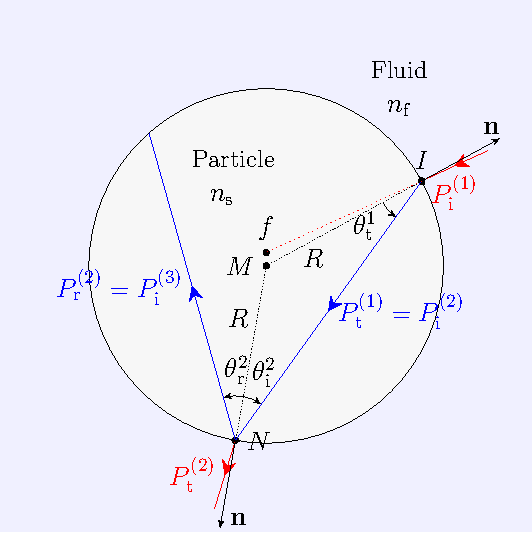
\includegraphics[]{/ray.pdf}
  \caption{Schematic of ray path through particle.}
  \label{fig:TO-ray_particle}
\end{figure}

With the convergence angle $\beta$ (see \cref{fig:TO-angles}) and the sine-law
\begin{equation}
  \frac{\sin\left( \frac{\pi}{2}-\beta \right)}{\R} = 
  \frac{\sin\incident}{\Rprime}
  \label{eq:TO-sine-law}
\end{equation}
one can compute $\incident$ as function of $\beta$. The angle $\beta$ is an 
input parameter and therefore known. The maximal convergence angle 
$\beta_{\MR{max}}$ is evaluated by the definition of the NA
\begin{equation}
  \cNA = \nf\,\sin\beta_{\MR{max}}.
  \label{eq:TO-NA}
\end{equation}
Our lens has a $\cNA$ of 1.27 and water has a refractive index of $\nf=1.33$ 
(see \cref{fig:TO-n_water}) and therefore our maximal convergence angle 
$\beta_{\MR{max}} \approx \SI{72}{\degree}$.

By knowing $\transmitted^{1}$ the path of the ray inside the particle is 
determined. At the next intersection point of the ray with the particle 
surface $N$, the ray is again partly transmitted into the fluid and partly 
reflected. Since the triangle $\bigtriangleup_{AMN}$ is an isosceles triangle 
(two sides have the same length $R$) and since per definition the reflected 
angle equals the incident angle, all internal reflection angles for one ray 
have the same magnitude ($\transmitted^{1}=\incident^{n}=\reflected^{n}$ for 
$n>1$).

Now, the respective powers of one ray can be evaluated. The ray has the 
incident power $\power{i}{1}$ with every reflection it gets split into two 
portions. With \cref{eq:TO-fresnelR,eq:TO-fresnelT,eq:TO-fresnel} the powers 
after each reflection is
\begin{subequations}
  \begin{alignat}{3}
    \power{t}{1} & = \fresnelT\left( \incident^{1} \right)\,\power{i}{1} && \\
    \power{r}{2} & = \fresnelR\left( \transmitted^{1} \right)\,\power{t}{1} && 
    = \power{i}{1}\,\fresnelT\left( \incident^{1} \right)\,
    \fresnelR\left( \transmitted^{1} \right) \\
    \power{t}{2} & = \fresnelT\left( \transmitted^{1} \right)\,\power{t}{1} && 
    = \power{i}{1}\,\fresnelT\left( \incident^{1} \right)\,
    \fresnelT\left( \transmitted^{1} \right) \\
    \power{r}{3} & = \fresnelR\left( \transmitted^{1} \right)\,\power{i}{3} && 
    = \power{i}{1}\,\fresnelT\left( \incident^{1} \right)\,
    \fresnelR^{2}\left( \transmitted^{1} \right).
\end{alignat}
\end{subequations}

\begin{figure}[thp]
  \centering
  % \tikzsetnextfilename{angles}

\tikzstyle arrowstyle=[scale=2]
\tikzstyle directed=[postaction={decorate,decoration={markings,
    mark=at position .65 with {\arrow[arrowstyle]{stealth}}}}]

\begin{tikzpicture}[scale=1.3]
    \coordinate (O) at (0,0);
    \coordinate (I) at (4,3);
    \coordinate (A) at (0,1.4);

    \node[circle,fill=black,inner sep=0pt,minimum size=3pt,label=below:{$M$}] 
    at (O) {};
    \node[circle,fill=black,inner sep=0pt,minimum size=3pt,label=left:{$f$}] at 
    (A) {};
    \node[circle,fill=black,inner sep=0pt,minimum size=3pt,label=above:{$I$}] 
    at (I) {};

    % \draw (O) -- node[midway, below, xshift=1mm] {$R$} (I) -- node[above, 
    % midway, xshift=-1mm] {$y$} (A) -- node[midway, left] {$a\,R$} cycle;
    \draw (O) -- node[midway, below, xshift=1mm] {$\R$} (I) -- (A) -- 
    node[midway, left] {$a\,\R$} cycle;

    % \draw[dotted] (O) rectangle (I);
    \draw[dotted] (A) -- ++(0,1);

    \draw[->,>=stealth'] (I) -- node[above,midway] {$\normalvector$} (36.86:6);

    \draw[directed,red] (34.0:6.2) -- (I);


    \draw[] (0,0.5) arc (90:37:0.5) node[midway, above] {$\gamma$};
    \draw[] (0,1.9) arc (90:22:0.5) node[midway, above] {$\beta$};
    \draw[] (0,1.1) arc (-90:22:0.3) node[midway, right] 
    {$\sfrac{\pi}{2}-\beta$};
    \draw[] (36.8:3.5) arc (216:200.5:1.5) node[pos=.3, left] {$\incident$};

    \draw[] (I) arc (36.86:48:5);
    \draw[] (I) arc (36.86:-3:5);

\end{tikzpicture}

  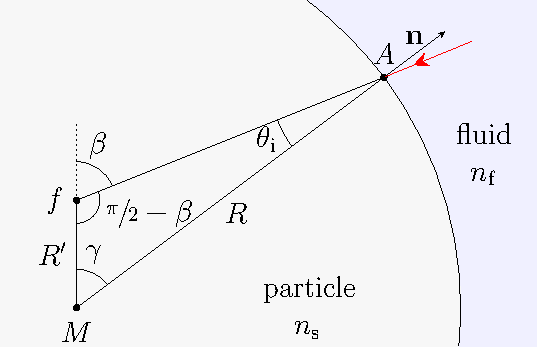
\includegraphics[]{/angles.pdf}
  \caption{Sketch of incident ray onto particle surface.}
  \label{fig:TO-angles}
\end{figure}

If a particle is stably trapped the distance $\Rprime$ is about $\Rprime 
\approx 0.1R$~\cite{Lamprecht2017}. During the trapping process and due to 
external forces this distances changes. If the focal point is outside the 
particle, the forces from the laser beam are too small to trap objects.

\cref{fig:TO-gamma_theta} depicts the values of $\gamma$ and $\incident$, 
respectively, for different combinations of $a$ and $\beta$. As pointed out 
before, the distance $\Rprime \approx 0.1\R$. For this distance the maximal 
incident angle $\incident$ over the whole range of $\beta$ is less than 
\SI{10}{\degree}.

\begin{figure}
  \centering
  \begin{subfigure}[b]{0.45\textwidth}
    \centering
    % \tikzsetnextfilename{gamma}
%%%%%%%
% READ TABLE
%%%%%%%

\begin{tikzpicture}
    \begin{axis}[view={0}{90},
        xlabel={$a$ [-]},
        ylabel={$\beta$ [\si{\degree}]},
        xmax=0.5,
        height=60mm,
        point meta min=0,
        point meta max=72,
        width=60mm,
        colormap/YlGnBu-9,
        colorbar,
        colorbar horizontal,
        colorbar style={
          title={$\gamma$ [\si{\degree}]},
          at={(0,1.3)},
          anchor=north west,
          xtick={0,24,48,72},
        },
        ytick={0,24,48,72},
        xtick={0,0.25,0.5},
      ]
      % countourf
      \addplot3[surf,mesh/rows=51,shader=interp] table[x=a,y=beta,z=gamma] 
      {\relPath/10_Figures/TikZ/angles_mat.dat};
      % lines
       \addplot3[
         mesh/rows=51,
         mesh/cols=50,
         contour gnuplot={levels={9,18,36,54},draw color=black},
     ] table[x=a,y=beta,z=gamma] {\relPath/10_Figures/TikZ/angles_mat.dat};

    \end{axis}
\end{tikzpicture}

    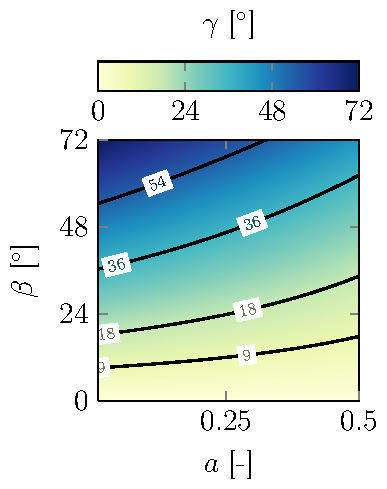
\includegraphics[]{/gamma.pdf}
    \caption{}
    \label{fig:TO-gamma}
  \end{subfigure}
  \hfill
  \begin{subfigure}[b]{0.45\textwidth}
    \centering
    % \tikzsetnextfilename{theta_i}
%%%%%%%
% READ TABLE
%%%%%%%

\begin{tikzpicture}
    \begin{axis}[view={0}{90},
        xlabel={$a$ [-]},
        ylabel={$\beta$ [\si{\degree}]},
        xmax=0.5,
        height=60mm,
        point meta min=0,
        point meta max=30,
        width=60mm,
        colormap name=viridis,
        colorbar,
        colorbar horizontal,
        colorbar style={
          title={$\incident$ [\si{\degree}]},
          at={(0,1.3)},
          anchor=north west,
          xtick={0,10,20,30},
        },
        ytick={0,24,48,72},
        xtick={0,0.25,0.5},
      ]
      \addplot3[surf,mesh/rows=51,shader=interp] table[x=a,y=beta,z=theta] 
      {\relPath/10_Figures/TikZ/angles_mat.dat};
    \end{axis}
\end{tikzpicture}

    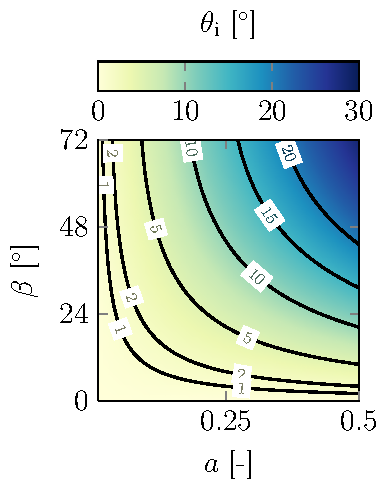
\includegraphics[]{/theta_i.pdf}
    \caption{}
    \label{fig:TO-theta_i}
  \end{subfigure}
    \caption{Magnitude of $\gamma$ and $\incident$ for different values of 
    $a=\nicefrac{\Rprime}{\R}$ and $\beta$ (see also \cref{fig:TO-angles}).}
  \label{fig:TO-gamma_theta}
\end{figure}

\begin{figure}[tbp]
  \centering
  % \tikzsetnextfilename{Fresnel}
%%%%%%%
% READ TABLE
%%%%%%%
\pgfplotstableread{\relPath/10_Figures/TikZ/Fresnel.dat}{\data}

\begin{tikzpicture}
  \begin{groupplot}[
    axis on top=true,
    group style={
      group size=2 by 1,
      horizontal sep = 23mm,
    },
    xmin=0,
    ymin=0,
    height=55mm,
    width=73mm,
    no markers,
  ]
  \nextgroupplot[
    xlabel={Incident angle $\incident$ [\si{\degree}]},
    ylabel={\footnotesize Fresnel Coefficient [-]},
    xtick={0,0.16666,0.333333,0.5},
    xticklabels={0, 30, 60, 90},
    legend style={
      at={(axis cs:0.01,0.5)},
      anchor=west,
      font=\footnotesize,
    }
  ]
  \filldraw[black!10!,opacity=0.7] (0.155,0) rectangle ({0.5,1}|-{rel axis 
  cs:1,1});

    \addplot[dashed] table[x=theta,y=R_M2P] {\data};
    \addlegendentry{$\fresnelR_{\mathrm{f\rightarrow s}}$};
    \addplot[] table[x=theta,y=T_M2P] {\data};
    \addlegendentry{$\fresnelT_{\mathrm{f\rightarrow s}}$};

    \addplot[thick, blue, dotted] table[x=theta,y=R_P2M] {\data};
    \addlegendentry{$\fresnelR_{\mathrm{s\rightarrow f}}$};
    \addplot[thick, blue] table[x=theta,y=T_P2M] {\data};
    \addlegendentry{$\fresnelT_{\mathrm{s\rightarrow f}}$};

    \nextgroupplot[
    xlabel={Incident angle $\incident$ [\si{\degree}]},
    xmax=0.167,
    ymin=0.001,
    ymode=log,
    xtick={0,0.05555,0.11111,0.1666666},
    xticklabels={0, 10, 20, 30},
  ]

  \filldraw[black!10!,opacity=0.7] (0.155,0.00001) rectangle ({0.167,1}|-{rel 
  axis cs:1,1});

    \addplot[dashed] table[x=theta,y=R_M2P] {\data};
    \addplot[] table[x=theta,y=T_M2P] {\data};

    \addplot[thick, blue, dotted] table[x=theta,y=R_P2M] {\data};
    \addplot[thick, blue] table[x=theta,y=T_P2M] {\data};

  \end{groupplot}
  % \draw[thick,blue,->,shorten >=2pt,shorten <=2pt] (group c1r1.east) -- (group 
  % c2r1.west);
\end{tikzpicture}

  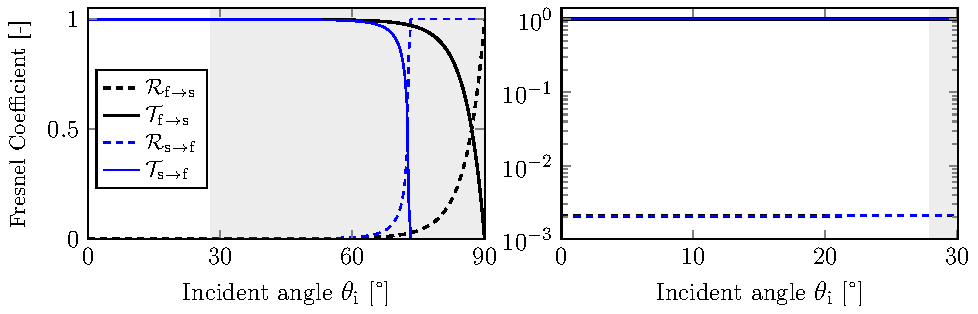
\includegraphics[]{/Fresnel.pdf}
  \caption{Fresnel coefficients of reflectance and transmittance (see 
    \cref{eq:TO-fresnelR,eq:TO-fresnelT}) for a fluid-solid interface 
    ($\Box_{\MR{f}\rightarrow\MR{s}}$) and a solid-fluid interface 
    ($\Box_{\MR{s}\rightarrow\MR{f}}$); $\nf=1.33$ and $\ns=1.42$. The right 
    plot is a detail of the left one with a logarithmic y-scale. The gray 
    shaded area marks the interval of incident angles $\incident$ that do not 
  occur in our setup.}
  \label{fig:TO-fresnel}
\end{figure}

Finally, we can estimate the total relative absorbed energy $\Xi$ by the 
particle. \cref{eq:TO-beer-lambert} defines the intensity of a single ray after 
a distance $s$. Hence the relative absorbed intensity over this length is
\begin{equation}
  \intensity_{\MR{abs}} = \intensity_{0} \left( 1 - \exp(-\alpha_{\MR{s}}\,s) 
  \right).
    \label{eq:TO-absorbed_energy}
\end{equation}
The distance $s$ for one passage through the particle can be computed as 
function of $\beta$ as
\begin{equation}
  s\left( \beta \right)
  =
  2R\,\cos\transmitted
  =
  2R\,\cos\left\{ \transmitted\left[ \incident\left( \beta \right) \right] 
  \right\}.
    \label{eq:TO-distance_s}
\end{equation}
And the power of a ray after $j$ reflections inside the particle is
\begin{equation}
  \begin{alignedat}{3}
    \power{i}{j} &=
    \power{i}{1} \, &&
    \fresnelT_{\MR{f}\rightarrow\MR{s}}\left( \incident \right) \, &&
    \left[\fresnelR_{\MR{s}\rightarrow\MR{f}}\left( \transmitted 
    \right)\right]^{(j)}\\
    &=
    \power{i}{1} \, &&
    \fresnelT_{\MR{f}\rightarrow\MR{s}}
    \left( \incident\left( \beta \right) \right) \, &&
    \left[
      \fresnelR_{\MR{s}\rightarrow\MR{f}}
      \left( \transmitted\left( \incident\left( \beta \right) \right) \right)
  \right]^{(j)} \coloneqq \power{i}{j}\left( \beta \right)
  \end{alignedat}
  \label{eq:TO-power}
\end{equation}
where $\Box_{\MR{f}\rightarrow\MR{s}}$ indicates fluid-solid interface and 
$\Box_{\MR{s}\rightarrow\MR{f}}$ the solid-fluid interface. With 
\cref{eq:TO-absorbed_energy,eq:TO-distance_s,eq:TO-power} the relative absorbed 
energy $\Xi$ inside the particle can be approximated with $N$ discrete values
\begin{equation}
  \beta_{n} = \frac{n}{N}\,\beta_{\MR{max}}\quad\text{with}\quad 
  n\in\left\{1,2,\ldots,N\right\}.
  \label{eq:TO-beta-disc}
\end{equation}
to be
\begin{equation}
    % \intensity_{\MR{tot.,abs.}} \approx
    \Xi \approx
    \frac{2\pi}{N}
    \sum\limits_{n=1}^{N}
    \sum\limits_{m=0}^{\infty}
    \left\{ 1 - \exp\left[-\alpha_{\MR{s}}\,s\left( \beta_{n} \right) \right] 
    \right\}
    \underbrace{\power{i}{m}\left( \beta_{n} \right)}_{
    \fresnelT_{\MR{f}\rightarrow\MR{s}}\left( \beta_{n}\right) \,
    \left[\fresnelR_{\MR{s}\rightarrow\MR{f}}\left(\beta_{n}\right)\right]^{(m)}
}
  \label{eq:TO-total-absorbed}
\end{equation}
where the factor $\nicefrac{1}{N}$ is due to the assumption that each ray has 
the same incident power when hitting the particle surface and the factor $2\pi$ 
for considering the full volume of the particle. Per definition the reflectance 
$\fresnelR$ and the transmittance $\fresnelT$ are smaller than 1. This property 
as well as
\begin{equation}
  \sum\limits^{\infty}_{m=0} \Box^{m} = \frac{1}{1-\Box}
  \quad\text{for}\quad\abs{\Box} < 1
\end{equation}
can be applied to \cref{eq:TO-total-absorbed} to simplify the double sum to
\begin{equation}
  % \intensity_{\MR{tot.,abs.}} \approx
  \Xi \approx
  \frac{2\pi}{N}
  \sum\limits_{n=1}^{N}
  \fresnelT_{\MR{f}\rightarrow\MR{s}}\left( \beta_{n} \right)
  \left[ 1 - \exp\left( -\alpha_{\MR{s}}\,s\left( \beta_{n} \right) \right) 
  \right]
  \,\frac{1}{1-\fresnelR_{\MR{s}\rightarrow\MR{f}}\left( \beta_{n} \right)}.
  \label{eq:TO-total-absorbed-simp}
\end{equation}

\cref{fig:TO-fresnel} depicts the values for $\fresnelT$ and $\fresnelR$ for 
the fluid-particle interface and the particle-fluid interface. Noteworthy is 
the fact, that for the occurring incident angles $\incident \leq 
\SI{10}{\degree}$ the values of $\fresnelR$ for both interface are less than 
$3\cdot 10^{-3}$. Therefore, most of the energy is transmitted and almost none 
reflected. For example, the relative power after one internal reflection and 
for an incident angle of $\incident=\SI{10}{\degree}$ is $\approx 2.07\cdot 
10^{-3}\,\power{i}{1}$ and after two internal reflections already $\approx 
4.31\cdot 10^{-6}\,\power{i}{1}$.

\begin{figure}[tbp]
  \centering
  % \tikzsetnextfilename{absorbed_energies}

\begin{tikzpicture}
  \begin{axis}[
      view={0}{90},
      ylabel={$\nicefrac{\Rprime}{\R}$ [-]},
      xlabel={$R$ [\si{\um}]},
      height=50mm,
      width=100mm,
      point meta min=0.2,
      point meta max=2.7,
      colorbar,
      colormap/BuPu-9,
      colorbar horizontal,
      colorbar style={
        title={\footnotesize Relative absorbed Energy $\Xi$ ($\times 
        10^{-4}$)},
        at={(0,1.4)},
        anchor=north west,
        xtick={0.2,0.5,1.0,1.5,2.0,2.5},
      },
    ]
      % contourf
      \addplot3[surf,mesh/rows=21,shader=interp] table[x=R,y=a,z=alpha] 
      {\relPath/10_Figures/TikZ/absorbed_energies.dat};
      % lines
       \addplot3[
         mesh/rows=21,
         mesh/cols=20,
         contour gnuplot={draw color=black},
     ] table[x=R,y=a,z=alpha] {\relPath/10_Figures/TikZ/absorbed_energies.dat};

  \end{axis}
\end{tikzpicture}

  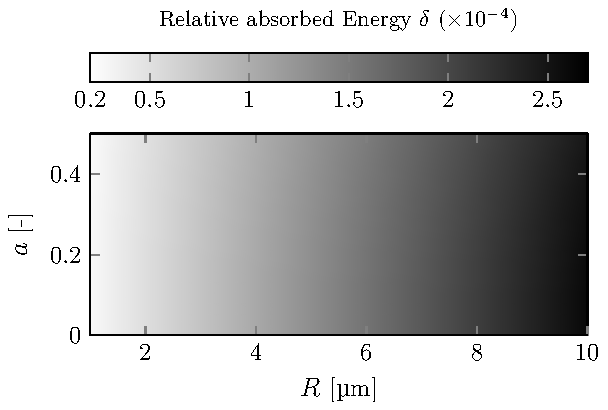
\includegraphics[]{/absorbed_energies.pdf}
  \caption{Results of \cref{eq:TO-total-absorbed-simp} of \SiO~for various 
  values of $\nicefrac{\Rprime}{\R}$ and radii $R$ with $N=500$. The optical 
absorption $\alpha_{\MR{s}}$ of \SiO~at $\lal=\SI{785}{\nm}$ is about 
\SI{2.08}{\per\meter}~\cite{Kitamura2007}.}
  \label{fig:TO-absorbed_energies}
\end{figure}

\cref{fig:TO-absorbed_energies} shows the relative absorbed energy $\Xi$ inside 
a particle for various radii $R$ and distances $\Rprime$. As 
\cref{fig:TO-fresnel} already suggested only a little fraction of the trapping 
energy is absorbed by the \SiO~particle itself with a refractive index of 
$\ns=1.42$.

\subsection{Ray Optics Heat Approximation}

With the knowledge of the relative absorbed energy $\Xi$ by the particle, we 
solve the heat equation for the particle
\begin{equation}
  \laplacian{T} = \frac{1}{\kappa} \pdv{T}{t} - \frac{q}{K}
  \label{eq:TO-heat-prob}
\end{equation}
where $T$ is the temperature inside the particle, $q$ is the absorbed energy 
per unit volume, $K$ the thermal conductivity, and $\kappa$ the thermal 
diffusivity. Going further, we neglect the time-dependence $\pdv{T}{t}= 0$ 
because all publications presented in \cref{sec:TO-state} state that the 
heating occurs within \si{\ms} and the temperature does not change afterwards 
anymore \begin{equation}
  \laplacian{T} = - \frac{q}{K}.
  \label{eq:TO-heat-stat}
\end{equation}
 In addition, we assume a spherical particle and solve the problem with a 
 spherical coordinate system (see \cref{fig:TA-coordinate}) with its origin at 
 the particle center. Additionally, we take the source term $q$ to be constant 
 throughout the particle. Therefore, we neglect all partial derivatives with 
 respect to the angles $\varphi$ and $\theta$ and solve a second order ordinary 
 differential equation
 \begin{equation}
    \frac{1}{r^{2}}\pdv{r}\left( r^{2}\pdv{T}{r} \right) = - \frac{q}{K}
  \label{eq:TO-heat-spherical}
\end{equation}
with only a $r$ dependence and a constant source term. We complete the problem, 
with two boundary conditions
\begin{subequations}
\begin{align}
  \eval{\pdv{T}{r}}_{r=0} &= 0 \label{eq:TO-heat-BC1}\\[3mm]
  \eval{T}_{r=\R} &= T_{0} \label{eq:TO-heat-BC2}.
\end{align}
\end{subequations}
The first one ensures that there is no heat flux in and out of a single point, 
the origin of the particle ($r=0$). And the second boundary condition fixes the 
temperature at the surface of the particle ($r=\R$). It implies that the 
temperature at the surface of the particle is constant and, therefore, neither 
the surrounding mediums is influenced by the temperature distribution of the 
particle nor vice-versa. Depending on the material properties of the particle 
and its resulting temperature increase this boundary condition might model a 
non-physical situation. However, for \SiO~the optical absorption coefficient 
$\alpha_{\MR{s}}$ is with a value of \SI{2.08}{\per\meter} at 
$\lal=\SI{785}{\nm}$~\cite{Kitamura2007} close to the absorption coefficient of 
water (\SI{2.144}{\per\meter}) and, therefore, only a small temperature 
increase is expected where the second boundary condition is still well 
applicable.

After two consecutive integration and the enforcement of the boundary 
conditions one finds the difference temperature to be
\begin{equation}
 \Delta T(r) = T(r) - T_{0} = \frac{q}{6K}\left(\R^2 - r^{2} \right).
  \label{eq:TO-heat-sol}
\end{equation}
The average temperature increase over the whole particle is the volume integral 
of \cref{eq:TO-heat-sol}
\begin{equation}
  \overline{\Delta T} = \frac{1}{V}\int_{V}\Delta T(r) \dd{V} = 
  \frac{1}{15}\,\frac{q}{K}\,R^{2}.
  \label{eq:TO-heat-avg}
\end{equation}
This can be further simplified since $q$ is the absorbed energy per unit volume
\begin{equation}
  q = \frac{\Xi\,P}{V} = \frac{3}{4}\,\frac{\Xi\,P}{\pi\,\R^{3}}
\end{equation}
where $P$ is the incident power of the laser and $V$ the volume of the 
particle. Finally, the average temperature increase of the spherical particle 
is
\begin{equation}
  \overline{\Delta T} = \frac{1}{20\,\pi}\,\frac{\Xi\,P}{\R\,K}.
  \label{eq:TO-heat-sol-simp}
\end{equation}
Interestingly, \cref{eq:TO-heat-sol-simp} seems to scale with $\propto 
\nicefrac{1}{\R}$. However, the relative total absorbed energy $\Xi$ is also 
dependent on $\R$ because the travelled distance of a ray within the 
particle $s$ increases with the particle size linearly. But $\Xi$ scales with 
$\left[  1-\exp\left( -\alpha_{\MR{s}}\,\R \right)\right]$ and therefore the 
average difference temperature $\overline{\Delta T}$ is proportional to 
$\nicefrac{\left[ 1-\exp\left( -\alpha_{\MR{s}}\,\R \right) \right]}{\R}$. This 
seems counter-intuitive, that a bigger particle size lead to less temperature 
increase. But it only holds for the average temperature difference 
$\overline{\Delta T}$, the maximal temperature distribution $T\vert_{r=0}$ 
(\cref{eq:TO-heat-sol}) increases with the particle size 
($T\vert_{r=0}\propto\R^{2}$).

\begin{figure}[tbp]
  \centering
  % \tikzsetnextfilename{dT}
%%%%%%%
% READ TABLE
%%%%%%%
\begin{tikzpicture}
    \begin{axis}[view={0}{90},
        xlabel={$R$ [\si{\um}]},
        ylabel={$P$ [\si{\milli\watt}]},
        height=60mm,
        width=100mm,
        point meta min=0,
        point meta max=70,
        colormap = {whitered}{
          color(0cm) = (white);
          color(1cm) = (red)},
        colorbar,
        colorbar style={
          ytick={0,35,70},
          ylabel={$\overline{\Delta T}$ [\si{\milli\degreeCelsius}]},
        },
        xtick={1,5,10},
      ]
      % contourf
      \addplot3[
        surf,
        mesh/rows=21,
        shader=interp
      ] table[x=R,y=P,z=dT] {\relPath/10_Figures/TikZ/dT.dat};
      % lines
       \addplot3[
         mesh/rows=21,
         mesh/cols=20,
         contour gnuplot={levels={15,30,45,60},draw color=black},
     ] table[x=R,y=P,z=dT] {\relPath/10_Figures/TikZ/dT.dat};
    \end{axis}
\end{tikzpicture}

  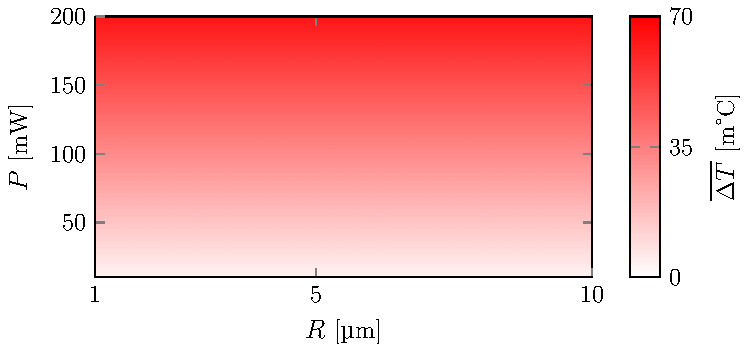
\includegraphics[]{/dT.pdf}
  \caption{$\overline{\Delta T}$ of \cref{eq:TO-heat-sol-simp} for various 
  laser powers $P$ and particle radii $R$; 
$K=\SI{1.4}{\watt\per\meter\per\kelvin}$ for \SiO.}
  \label{fig:TO-dT}
\end{figure}

\Cref{fig:TO-dT} depicts the average difference temperature for various 
combinations of laser power $P$ and particle radius $R$. With the information 
given in the aforementioned experimental studies regarding the heating by the 
laser and these ray optics motivated results for the heat distribution inside 
the particle, we conclude that the increase in temperature around and inside 
the particle for our setup is less than \SI{2}{\degreeCelsius} with the applied 
laser power in the low \si{\milli\watt} range. The main part is by the 
absorption of the fluid around the particle \begin{equation}
  \Delta T_{\MR{fluid}}
  \leq
  \SI{0.2}{\watt}\cdot\SI{10}{\celsius\per\watt}
  =
  \SI{2}{\celsius}
\end{equation}
with a maximal available laser power of \SI{200}{\milli\watt} for our setup and 
the \SiO~particle gets only further heated by values smaller than 
\SI{70}{\milli\celsius}.

Having established an upper bound for the laser induced temperature increase 
for water and \SiO~particles, we can estimate the effects of the temperature 
increase to the absolute value of a measured force with the OT. The parameter 
that changes the most by a change in the temperature is the dynamic viscosity 
$\muef$ of the fluid. The viscosity is in general a function of the temperature 
$\muef\coloneqq\muef(T)$. For our calibration routine the absolute measured 
force of the OT scales with square root of the fluid viscosity 
($\abs{\vb{\force}}\propto\sqrt{\muef}$). For the range of 
\SIrange{20}{30}{\degreeCelsius} the dynamic viscosity of water (exact formula 
from \cite{Peterman2003}) can be linearly approximated with
\begin{equation}
  \muef(T) = 8.9086\cdot 10^{-4} -2.0277\cdot10^{-5} (T-25).
  \label{eq:TO-viscosity}
\end{equation}
Temperature deviations of $\SI{25}{\degreeCelsius}\pm\SI{2}{\degreeCelsius}$ 
lead to force magnitude errors of less than $\pm$2.5\%. This percentage is 
acceptable small such that we neglect the temperature induced viscosity change 
and use the ambient room temperature as reference.

For a different particle material, e.g. copper, with material parameters of 
$\nreal_{\MR{Cu}}=0.24891$~\cite{Johnson1972}, 
$\alpha_{\MR{Cu}}(\SI{785}{\nm})\approx\SI{7.8e7}{\per\meter}$~\cite{Johnson1972}, 
and $K_{\MR{Cu}}=\SI{398}{\watt\per\meter\per\kelvin}$, the average temperature 
increase $\overline{\Delta T}_{\MR{cu}}$ using the simplified stationary heat 
equation with a laser power of \SI{100}{\milli\watt}, a particle radius of 
\SI{1.03}{\um}, and $\Rprime=0.1$ is about \SI{24}{\degreeCelsius}. With such a 
large temperature increase just by the particle the stationary heat equation is 
not able to fully capture the underlying physics. The heat flux at the particle 
surface into the surrounding medium is accounted for by the second boundary 
condition (\cref{eq:TO-heat-BC2}). For particle materials which are much more 
absorbing as the surrounding medium, numerical simulation need to be 
implemented to calculate the laser induced heating and the subsequent viscosity 
change.

\section{Optical Position Detection\label{sec:TO-QPD}}

Besides trapping objects, the OT can also measure the relative movement of the 
trapped object within the trap. After a calibration of the OT, it is possible 
to convert the movement into the physical unit of meter and then also convert 
it into a force with unit Newton. Besides tracking the movement visually with, 
e.g., a high-speed camera, the most common approach is to utilize QPDs. The 
latter is superior to the camera because higher sampling rates are 
straightforward to achieve, less data is produced during the measurement and a 
full three dimensional resolution is possible.

In order to do so, the laser beam must be collimated after the object trapping 
region and then focussed with separate lenses onto two QPDs (see 
\cref{fig:TO-setup}). While the laser beam is focussed within the aperture of 
the QPD for the in-plane $xy$-direction (QPDxy), the beam is focussed to 
overfill the QPD aperture for the $z$-direction. For all measurements, where 
the measured signals of the QPDs needs to be converted to meter, it is crucial 
to operate in the so-called \emph{linear regime} of the QPD. In the following, 
we will show what the linear regime is.

A QPD consists of a diode divided into four separate regions. Each of the four 
diodes measures the intensity of light on its respective area and returns a 
measure in voltage. The QPD has an aperture opening radius $R_{\MR{QPD}}$. 
\cref{fig:TO-QPD} is a schematic of the QPDxy where the focussed laser spot 
midpoint $M$ is at $x=x_{0}$ and $y=y_{0}$ and the radius of the laser spot is 
about $\sfrac{1}{5}\,R_{\MR{QPD}}$~\cite{Lamprecht2017}.

The normalized intensity distribution of the laser can be modeled as
\begin{equation}
  \tilde{\intensity} = \tilde{\intensity}(x, y) = 
  \frac{1}{2\pi\,R_{\MR{spot}}^{2}}\,\exp\left[ 
  -\frac{1}{2}\,\frac{(x-x_{0})^{2} + (y - y_{0})^{2}}{R_{\MR{spot}}^{2}} 
\right]
    \label{eq:TO-intensity}
\end{equation}
where the radius of the spot is $R_{\MR{spot}}=\sfrac{\RA}{5}$ and the property 
\begin{equation}
  \int\limits_{\dd{A}}\tilde{\intensity}\dd{A} = 1
\end{equation}
holds.

\begin{figure}[tbp]
  \centering
  % \tikzsetnextfilename{QPD}
%%%%%%%
% READ TABLE
%%%%%%%

\begin{tikzpicture}

  \coordinate (M) at (-1.5, 0.2);


  \draw[<->,latex-latex] (0, 3.5) -- node[above,pos=0] {$\ey$} (0,0) -- 
  node[above,pos=1] {$\ex$}  (3.5, 0);


  \draw[thick, black] (0,0) circle (3);
  \draw[|latex-{latex}|] (-3, -3.5) -- node[below,midway] {$2\,R_{\MR{QPD}}$} 
  ++(6,0);

  \draw[thick, dotted, black] (-3,0) -- ++(6,0);
  \draw[thick, dotted, black] (0,-3) -- ++(0,6);

  \draw[dotted, thick, red, fill=red!50, opacity=0.3] (M) circle (1);
  \draw[|latex-{latex}|] (-2.5, -1.5) -- node[above,midway] {$\approx 
  \sfrac{2}{5}\,R_{\MR{QPD}}$} ++(2,0);

  \fill (M) circle (0.5mm);
  \node[yshift=3mm,right] at (M) {$M$};
  \draw[thin] (M) -- node[pos=1,right] {\small$y_{0}$} ++(1.5,0);
  \draw[thin] (M) -- node[pos=1,below] {\small$x_{0}$} ++(0,-0.2);


  \foreach \angle [count = \xi] in {60,120,240,300}
  {
    \node at (\angle:2.7) {$V_{\xi}$};
  }

\end{tikzpicture}

  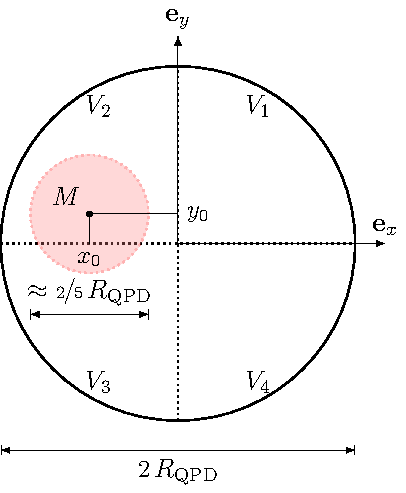
\includegraphics[]{/QPD.pdf}
  \caption{Sketch of quadrant photo detectors for $x$-$y$ detection with the 
  center of the laser image $M$ at $(x_{0}, y_{0})$.}
  \label{fig:TO-QPD}
\end{figure}

The measured voltage $V_{i}$ per quadrant is proportional to the received 
power. The received power per quadrant is the surface integral of the laser 
intensity. The four separate voltages can be evaluated with four integrals over 
the respective areas of the quadrants
\begin{subequations}
\begin{align}
  V_{\MR{1}} & \propto \int_{0}^{\sfrac{\pi}{2}}\int_{0}^{\RA}
  \tilde{\intensity}\left( r\cos\varphi, r\sin\varphi 
  \right)\,r\,\dd{r}\dd{\varphi}
  \label{eq:TO-V1}
  \\[3mm]
  V_{\MR{2}} & \propto \int_{\sfrac{\pi}{2}}^{\pi}\int_{0}^{\RA}
  \tilde{\intensity}\left(r\cos\varphi, 
  r\sin\varphi\right)\,r\,\dd{r}\dd{\varphi}
  \label{eq:TO-V2}
  \\[3mm]
  V_{\MR{3}} & \propto \int_{\pi}^{\sfrac{3\pi}{2}}\int_{0}^{\RA}
  \tilde{\intensity}\left(r\cos\varphi, 
  r\sin\varphi\right)\,r\,\dd{r}\dd{\varphi}
  \label{eq:TO-V3}
  \\[3mm]
  V_{\MR{4}} & \propto \int_{\sfrac{3\pi}{2}}^{2\pi}\int_{0}^{\RA}
  \tilde{\intensity}\left(r\cos\varphi, 
  r\sin\varphi\right)\,r\,\dd{r}\dd{\varphi}
  \label{eq:TO-V4}
\end{align}
\end{subequations}
where we used polar integration and polar coordinates $x=r\cos\varphi$ and 
$y=r\sin\varphi$.

\begin{figure}[tbp]
  \centering
  % \tikzsetnextfilename{V_quadrant}
%%%%%%%
% READ TABLE
%%%%%%%
\pgfplotstableread{\relPath/10_Figures/TikZ/V_mat.dat}{\data}

\renewcommand{\tikzHelper}{
  \draw[black] (-1,0,0)--(1,0,0);
  \draw[black] (0,-1,0)--(0,1,0);
  \draw[black] (0,0,0) circle (1);
  }

\pgfplotsset{%
    colormap={bwr}{
      color=(blue);
      color=(white);
      color=(red);
    }%
}
%%%%%%%%%%%%%%%%%%%%%%%%%%%%%%%%%%
% Voltages per Quadrant
%%%%%%%%%%%%%%%%%%%%%%%%%%%%%%%%%%

\begin{tikzpicture}
  \begin{groupplot}[view={0}{90},
    % xlabel=$x$,
    % ylabel=$y$,
    height=5cm,
    width=5cm,
    point meta min=0,
    point meta max=1,
    colormap={}{ gray(0cm)=(1); gray(1cm)=(0);},
    group/xlabels at = edge bottom,
    group style = {
      group size = 2 by 2,
      horizontal sep=5mm,
      vertical sep=5mm,
      xlabels at = edge bottom,
      ylabels at = edge bottom
    }]

    \nextgroupplot[
      xticklabels={,,},
      ylabel={$\sfrac{y_{0}}{\RA}$},
    ]
        \addplot3[surf,mesh/rows=99,shader=interp] table[x=x,y=y,z=V4] {\data};
        \tikzHelper

    \nextgroupplot[
      yticklabels={,,},
      xticklabels={,,},
      colorbar right,
      every colorbar/.append style={
        ylabel={Normalized Voltage $\normalized{V}$},
        height=2*\pgfkeysvalueof{/pgfplots/parent axis height}+
        \pgfkeysvalueof{/pgfplots/group/vertical sep}}]
        \addplot3[surf,mesh/rows=99,shader=interp] table[x=x,y=y,z=V1] {\data};
        \tikzHelper

    \nextgroupplot[
      xlabel={$\sfrac{x_{0}}{\RA}$},
      ylabel={$\sfrac{y_{0}}{\RA}$},
    ]
        \addplot3[surf,mesh/rows=99,shader=interp] table[x=x,y=y,z=V3]
        {\data};
        \tikzHelper

    \nextgroupplot[
      xlabel={$\sfrac{x_{0}}{\RA}$},
      yticklabels={,,},
    ]
        \addplot3[surf,mesh/rows=99,shader=interp] table[x=x,y=y,z=V2] {\data};
        \tikzHelper


  \end{groupplot}
\end{tikzpicture}

  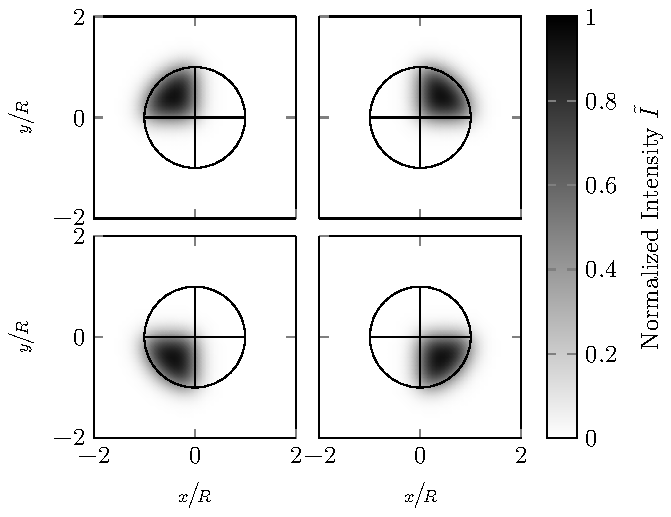
\includegraphics[]{/V_quadrant.pdf}
  \caption{Normalized voltage per quadrant for various positions of laser image 
  middle point $M$ (see \cref{eq:TO-V1,eq:TO-V2,eq:TO-V3,eq:TO-V4}). The top 
right plot is $V_{1}$, top left $V_{2}$, bottom left $V_{3}$, bottom right 
$V_{4}$.}
  \label{fig:TO-quadrant_Intensity}
\end{figure}

If the particle moves within the trap, the center of the laser image $M$ on the 
QPDxy also moves. \cref{fig:TO-quadrant_Intensity} shows the intensity per 
quadrant for different center positions. As expected, each quadrant is 
measuring the highest intensity whenever most of the laser image is over the 
respective area.

With these four separate values for $V_{1}$ through $V_{4}$, one can create a 
measure that is proportional to the movement of the laser image center $M$ 
along the $\ex$- and $\ey$-direction, respectively. These measures are 
additions and subtractions of the quadrants along one direction
\begin{subequations}
\begin{align}
  V_{\MR{x}} & = \left( V_{\MR{1}}+V_{\MR{4}} \right) - \left( V_{\MR{2}} + 
  V_{\MR{3}}  \right)
  \label{eq:TO-Vx} \\
  V_{\MR{y}} & = \left( V_{\MR{1}}+V_{\MR{2}} \right) - \left( V_{\MR{3}} + 
  V_{\MR{4}}  \right)
  \label{eq:TO-Vy} \\
  V_{\MR{t}} & = V_{\MR{1}}+V_{\MR{2}} + V_{\MR{3}} + V_{\MR{4}}.
  \label{eq:TO-Vt}
\end{align}
\end{subequations}

 \begin{figure}
  \centering
  \begin{subfigure}[b]{0.36\textwidth}
    \centering
    % \caption{$V_{\MR{x}}$}
    % \tikzsetnextfilename{QPDx}

\renewcommand{\tikzHelper}{
  \draw[black] (-1,0,0)--(1,0,0);
  \draw[black] (0,-1,0)--(0,1,0);
  \draw[black] (0,0,0) circle (1);

  \draw[black, dotted] (-1.5,0,0) -- (1.5,0,0);
  \draw[black, dotted] (-1.5,-0.6,0) -- (1.5,-0.6,0);
  \draw[black, dotted] (-1.5,0.6,0) -- (1.5,0.6,0);
}

\begin{tikzpicture}
  \begin{axis}[view={0}{90},
      xlabel=$\sfrac{x_{0}}{\RA}$,
      ylabel=$\sfrac{y_{0}}{\RA}$,
      point meta min=-1,
      point meta max=1,
      height=48mm,
      width=48mm,
      colormap/PuOr-11,
      colorbar,
      colorbar horizontal,
      colorbar style={
        title={\footnotesize Normalized Voltage $\normalized{V}_{x}$},
        at={(0,1.4)},
        anchor=north west,
        xtick={-1,0,1},
      }
    ]
      \addplot3[surf,mesh/rows=99,shader=interp] table[x=x,y=y,z=Vy] 
      {\relPath/10_Figures/TikZ/V_mat.dat};
    \tikzHelper
  \end{axis}
\end{tikzpicture}

    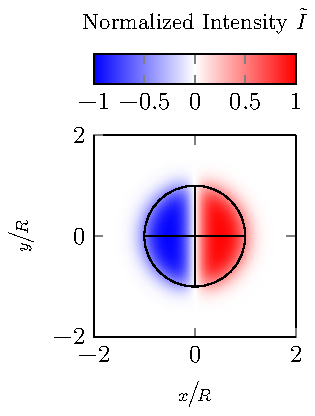
\includegraphics[]{/QPDx.pdf}
    \label{fig:TO-QPDx}
  \end{subfigure}
  \hfill
  \begin{subfigure}[b]{0.3\textwidth}
    \centering
    % \caption{$V_{\MR{y}}$}
    % \tikzsetnextfilename{QPDy}

\renewcommand{\tikzHelper}{
  \draw[black] (-1,0,0)--(1,0,0);
  \draw[black] (0,-1,0)--(0,1,0);
  \draw[black] (0,0,0) circle (1);
}

\pgfplotsset{%
    colormap={bwr}{
      color=(blue);
      color=(white);
      color=(red);
    }%
}

\begin{tikzpicture}
  \begin{axis}[view={0}{90},
      xlabel=$\sfrac{x}{\R}$,
      yticklabels={,,},
      point meta min=-1,
      point meta max=1,
      height=50mm,
      width=50mm,
      colorbar,
      colorbar horizontal,
      colorbar style={
        title={\footnotesize Normalized Intensity $\normalized{\intensity}$},
        at={(0,1.4)},
        anchor=north west,
        xtick={-1,-0.5,...,1},
      }
    ]
      \addplot3[surf,mesh/rows=51,shader=interp] table[x=x,y=y,z=Vx] 
      {\relPath/10_Figures/TikZ/V_mat.dat};
    \tikzHelper
  \end{axis}
\end{tikzpicture}

    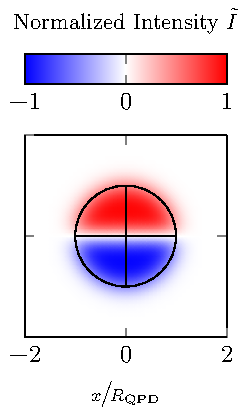
\includegraphics[]{/QPDy.pdf}
    \label{fig:TO-QPDy}
  \end{subfigure}
  \hfill
  \begin{subfigure}[b]{0.3\textwidth}
    \centering
    % \caption{$V_{\MR{t}}$}
    % \tikzsetnextfilename{QPDt}

\begin{tikzpicture}
  \begin{axis}[view={0}{90},
      xlabel=$\sfrac{x_{0}}{\RA}$,
      yticklabels={,,},
      height=48mm,
      width=48mm,
      colormap name=WhiteOr,
      colorbar,
      colorbar horizontal,
      colorbar style={
        title={\footnotesize Normalized Voltage $\normalized{V}_{t}$},
        at={(0,1.4)},
        anchor=north west,
        xtick={0,0.5,1},
      }
    ]
      \addplot3[surf,mesh/rows=99,shader=interp] table[x=x,y=y,z=V] 
      {\relPath/10_Figures/TikZ/V_mat.dat};

  \draw[black] (-1,0,0)--(1,0,0);
  \draw[black] (0,-1,0)--(0,1,0);
  \draw[black] (0,0,0) circle (1);

  \draw[black, dotted] (-1.5,0,0) -- (1.5,0,0);
  \draw[black, dotted] (-1.5,-0.6,0) -- (1.5,-0.6,0);
  \draw[black, dotted] (-1.5,0.6,0) -- (1.5,0.6,0);
  \end{axis}
\end{tikzpicture}

    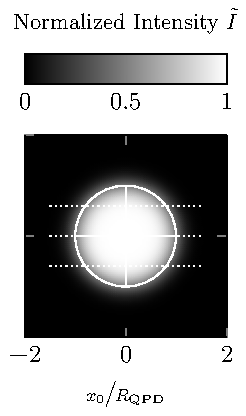
\includegraphics[]{/QPDt.pdf}
    \label{fig:TO-QPDt}
  \end{subfigure}
  \caption{QPD measure $\normalized{V}_{\MR{x}}$ (left;~\cref{eq:TO-Vx}), 
    $\normalized{V}_{\MR{y}}$ (center;~\cref{eq:TO-Vy}), and 
    $\normalized{V}_{\MR{t}}$ (right;~\cref{eq:TO-Vt}) for various positions of 
    laser image middle point $M$. Each plot is normalized to the maximal value 
  of $V_{\MR{t}}$. The dotted horizontal lines are at 
$y=\sfrac{-0.6}{R_{\MR{QPD}}}$, $y=\sfrac{0}{R_{\MR{QPD}}}$, and 
$y=\sfrac{0.6}{R_{\MR{QPD}}}$ respectively.}
  \label{fig:TO-QPDs}
 \end{figure}

As for the measured intensity per quadrant, the measured values are highest if 
the laser image is over the respective quadrants (see \cref{fig:TO-QPDs}). 
However, since the to the maximal value of $V_{\MR{t}}$ normalized 
$\normalized{V}_{\MR{x}}$ and $\normalized{V}_{\MR{y}}$ are composed by 
addition and subtraction of the strictly positive values $V_{i}$ the magnitude 
can now also be negative.

In \cref{fig:TO-voltages_over_x} the three measures are plotted over $x_{0}$ 
for three fixed values of $y_{0}$. This plot looks the same if $x_{0}$ is fixed 
and $y_{0}$ is the changing variable. Additionally the curves 
$\normalized{V}_{\MR{x}}$ and $\normalized{V}_{\MR{y}}$ change their behavior. 
There is a linear region for which a small movement of the laser image middle 
point $M$ is converted into a proportional change in the measured intensity on 
the QPD. However, this linear regime from $-0.15\,R_{\MR{QPD}}$ to 
$0.15\,R_{\MR{QPD}}$ is rather small. Therefore, it is very important to check 
and adjust the laser spot center position $M$ to be in the middle of the QPD 
before each measurement to ensure interpretability of the results.

Noteworthy is that for values of $\sfrac{\abs{x_{0}}}{R_{\MR{QPD}}} > 0.5$ a 
further outwards movement does not lead to an increase of the respective 
measure but to a decrease. If just one of the voltages, here $V_{\MR{y}}$, is 
taken into account then this decrease ($\sfrac{x_{0}}{R_{\MR{QPD}} > 0.5}$) is 
not distinguishable from the increase coming from the middle 
($\sfrac{x_{0}}{R_{\MR{QPD}} < 0.5}$). However, by also looking at the 
evolution of $\normalized{V}_{\MR{t}}$ it is possible to identify in which 
direction the laser image is moving on the QPD because this measure does not 
change its magnitude for $\abs{x_{0}} < 0.5\,R_{\MR{QPD}} $.

\begin{figure}[tbp]
  \centering
  % \tikzsetnextfilename{voltages_over_x}
%%%%%%%
% READ TABLE
%%%%%%%
\pgfplotstableread{\relPath/10_Figures/TikZ/V_line.dat}{\data}

\renewcommand{\tikzHelper}{
  \filldraw[black!10!, opacity=0.5] (-1,-1.1) rectangle (1,1.1);
}

\begin{tikzpicture}
\begin{groupplot}[
    group style={
        group name=myplot,
        group size= 1 by 3,
        vertical sep=8mm,
        },
    height=40mm,
    width=120mm,
    ymin=-1.1,
    ymax=1.1,
    ]
    \nextgroupplot[
    % ylabel={$\tilde{I}$},
      xticklabels={,,},
      title={$y = \sfrac{-0.64}{\RA}$},
      title style={yshift=-2mm},
      ]
      \tikzHelper
      \addplot[dotted] table[x=x,y=Vx_1] {\data};
      \addlegendentry{$V_{\MR{x}}$};
      \addplot[] table[x=x,y=Vy_1] {\data};
      \addlegendentry{$V_{\MR{y}}$};
      \addplot[dashed] table[x=x,y=V_1] {\data};
      \addlegendentry{$V_{\MR{t}}$};
    \nextgroupplot[
      % ylabel={$\tilde{I}$},
      title={$y = \sfrac{0}{\RA}$},
      title style={yshift=-2mm},
      xticklabels={,,},
      ylabel={Normalized Intensity $\normalized{\intensity}$},
      every axis y label/.append style={at=(ticklabel cs:0.5)}
      ]
      \tikzHelper
      \addplot[dotted] table[x=x,y=Vx_2] {\data};
      \addplot[] table[x=x,y=Vy_2] {\data};
      \addplot[dashed] table[x=x,y=V_2] {\data};
    \nextgroupplot[
      % ylabel={$\tilde{I}$},
      xlabel={$\sfrac{x}{\RA}$},
      title={$y = \sfrac{0.64}{\RA}$},
      title style={yshift=-2mm},
      ]
      \tikzHelper
      \addplot[dotted] table[x=x,y=Vx_3] {\data};
      \addplot[] table[x=x,y=Vy_3] {\data};
      \addplot[dashed] table[x=x,y=V_3] {\data};
\end{groupplot}
\end{tikzpicture}

  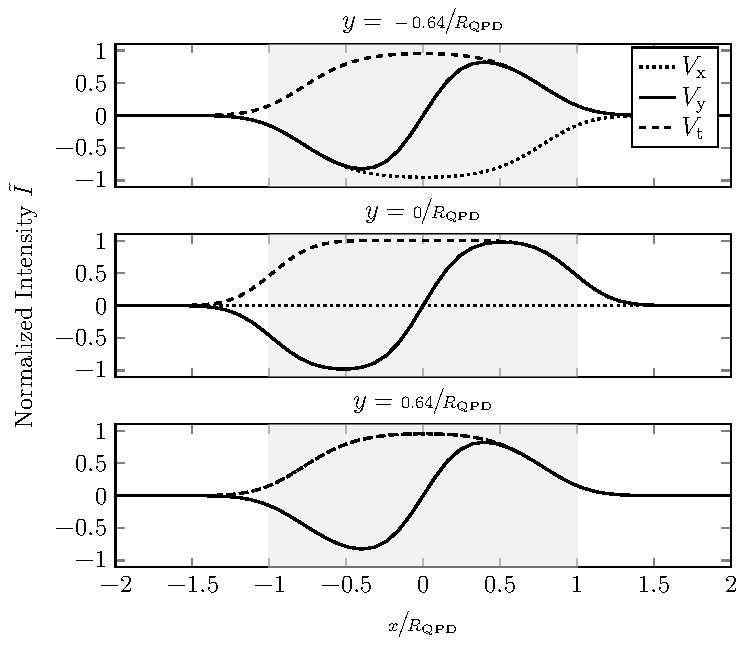
\includegraphics[]{/voltages_over_x.pdf}
  \caption{QPD measure $\normalized{V}_{\MR{x}}$ (\cref{eq:TO-Vx}), 
    $\normalized{V}_{\MR{y}}$
    (\cref{eq:TO-Vy}), and $\normalized{V}_{\MR{t}}$ (\cref{eq:TO-Vt}) over 
  $x_{0}$ for three fixed values of $y_{0}$. The light shaded gray area marks 
the boundaries of the QPD and the dark shaded gray area the linear region of 
the QPD from $-0.15\,R_{\MR{QPD}}$ to $0.15\,R_{\MR{QPD}}$.}
  \label{fig:TO-voltages_over_x}
\end{figure}
